% ============================================================
%  Reuters C50 — Klasifikacija autora novinskih tekstova
%  Seminarski rad — Istraživanje podataka
% ============================================================
\documentclass[12pt, a4paper]{article}

\usepackage[utf8]{inputenc}
\usepackage[T1]{fontenc}
\usepackage[serbian]{babel}
\usepackage{geometry}
\geometry{a4paper, margin=2.5cm}

\usepackage{graphicx}
\graphicspath{{./slike/}}
\usepackage{float}
\usepackage{caption}
\usepackage{subcaption}
\usepackage{booktabs}
\usepackage{array}
\usepackage{longtable}
\usepackage{multirow}
\usepackage{xcolor}
\usepackage{colortbl}
\usepackage{amsmath}
\usepackage{amssymb}
\usepackage{hyperref}
\hypersetup{
    colorlinks=true,
    linkcolor=blue!60!black,
    urlcolor=blue!60!black,
    citecolor=green!50!black
}
\usepackage{listings}
\usepackage{enumitem}
\usepackage{titlesec}
\usepackage{fancyhdr}
\usepackage{setspace}
\usepackage{parskip}
\usepackage{abstract}

% Stil za naslove sekcija
\titleformat{\section}{\large\bfseries\color{blue!70!black}}{}{0em}{\thesection\quad}
\titleformat{\subsection}{\normalsize\bfseries\color{blue!50!black}}{}{0em}{\thesubsection\quad}

% Stil za zaglavlje/podnožje
\setlength{\headheight}{14pt}
\pagestyle{fancy}
\fancyhf{}
\rhead{\small Reuters C50 --- Klasifikacija autora}
\lhead{\small Seminarski rad}
\cfoot{\thepage}
\renewcommand{\headrulewidth}{0.4pt}

% Definicija boja za tabele
\definecolor{rowgray}{RGB}{245,245,245}

\onehalfspacing

% Naslovna strana stilom \maketitle
\title{%
  \textbf{Authorship Classification}\\[0.4cm]
  \large Seminarski rad u okviru kursa\\
  Istra\v{z}ivanje podataka 2\\
  Matemati\v{c}ki fakultet
}
\author{Zagorka Pantovi\'{c}\\[0.1cm]
  \small mi20227@alas.matf.bg.ac.rs}
\date{Avgust 2026.}

% ============================================================
\begin{document}

\maketitle
\thispagestyle{empty}

% ============================================================
%  SAŽETAK
% ============================================================
\begin{abstract}
U ovom radu analiziran je problem identifikacije autora teksta kori\v{s}\'{c}enjem
metoda ma\v{s}inskog u\v{c}enja (eng.\ \textit{machine learning}). Cilj istra\v{z}ivanja
je razvoj modela koji na osnovu teksta novinskog \v{c}lanka mo\v{z}e da predvidi
njegovog autora.

Kori\v{s}\'{c}en je skup podataka Reuters~C50 koji sadr\v{z}i 5000 novinskih
\v{c}lanaka napisanih od strane 50 razli\v{c}itih autora. Rad obuhvata kompletnu
analiti\v{c}ku proceduru koja uklju\v{c}uje analizu podataka, obradu teksta,
ekstrakciju atributa pomo\'{c}u TF-IDF metode, vizualizaciju u 2D i 3D prostoru,
kao i treniranje i evaluaciju sedam klasifikacionih algoritama na tri razli\v{c}ita
skupa atributa (ukupno 21 model).

Testirani su: Multinomial Naive Bayes, Complement Naive Bayes, Logistic Regression,
Linear Support Vector Machine, K-Nearest Neighbors, Random Forest i Decision Tree.
Rezultati pokazuju da Linear SVM posti\v{z}e najbolje performanse sa ta\v{c}no\v{s}\'{c}u
klasifikacije od \textbf{72.4\%} na punom skupu od 10\,000 TF-IDF atributa.

Eksperimenti su tako{\dj}e pokazali da redukcija broja atributa sa 10\,000 na 2\,000
ima minimalan uticaj na performanse linearnih modela (pad od svega $\approx$1.5~pp),
dok dalje smanjenje na 500 atributa dovodi do primetnog pada ta\v{c}nosti kod svih algoritama.
\end{abstract}

% ============================================================
%  SADRŽAJ
% ============================================================
\newpage
\tableofcontents
\newpage

% ============================================================
%  1. UVOD
% ============================================================
\section{Uvod}

Ovaj seminarski rad bavi se problemom \textbf{klasifikacije autora novinskih tekstova} primenom
metoda mašinskog učenja nad Reuters C50 datasetom. Cilj je izgraditi model koji može da prepozna
autora članka na osnovu samog teksta, bez ikakvih metapodataka.

Atribucija autorstva teksta (\textit{authorship attribution}) je klasičan problem u obradi
prirodnog jezika koji ima primene u forenzičkoj lingvistici, detekciji plagijata i analizi
stilometrike. Ključni izazov leži u tome što različiti autori mogu pisati o sličnim temama,
pa model mora da nauči stilske, a ne samo tematske razlike.

U ovom radu:
\begin{itemize}
    \item Analiziramo i vizualizujemo Reuters C50 dataset,
    \item Primenjujemo preprocesiranje teksta (uklanjanje stop-reči, stemovanje),
    \item Vektorizujemo tekstove pomoću TF-IDF metode sa tri različita skupa atributa,
    \item Treniramo i poredimo \textbf{7 klasifikatora} na \textbf{3 skupa atributa} (ukupno 21 model),
    \item Evaluiramo modele pomoću višestrukih metrika i cross-validacije,
    \item Analiziramo koje atribute (reči) modeli smatraju najvažnijim.
\end{itemize}

Celokupan kod napisan je u programskom jeziku Python i organizovan u 5 Jupyter notebook-ova.

% ============================================================
%  2. OPIS PODATAKA
% ============================================================
\section{Opis podataka}

\subsection{Reuters C50 dataset}

Reuters C50 dataset potiče sa UCI Machine Learning Repository-ja
(\url{https://archive.ics.uci.edu/dataset/217/reuter+50+50}).
Sadrži novinske članke Reuters novinarske agencije, napisane od strane 50 različitih novinara.

\begin{table}[H]
\centering
\caption{Osnovne karakteristike Reuters C50 dataseta}
\begin{tabular}{ll}
\toprule
\textbf{Karakteristika}     & \textbf{Vrednost} \\
\midrule
Ukupan broj dokumenata      & 5000 \\
Broj autora (klasa)         & 50 \\
Dokumenti za trening        & 2500 (50 po autoru) \\
Dokumenti za testiranje     & 2500 (50 po autoru) \\
Tip podataka                & Tekstualni fajlovi (.txt) \\
Prosečan broj reči          & 505.7 reči/dokumentu \\
Prosečan broj karaktera     & 3102.9 kar./dokumentu \\
Ciljni atribut              & Ime autora (50 kategorija) \\
\bottomrule
\end{tabular}
\end{table}

Dataset je organizovan u dva foldera: \texttt{C50train} (trening skup) i \texttt{C50test}
(test skup). Unutar svakog foldera postoji po jedan podfolder za svakog od 50 autora,
a u njemu tačno 50 tekstualnih fajlova. Ovakva organizacija garantuje \textbf{savršeno
balansiran dataset} — svaka klasa ima identičan broj instanci.

Lista autora obuhvata novinare različitog porekla i geografskog fokusa:
anglosaksonski dopisnici (AaronPressman, BradDorfman), azijski dopisnici
(FumikoFujisaki, BenjaminKangLim, JaneMacartney, WilliamKazer),
evropski dopisnici (JanLopatka, JohnMastrini) i mnogi drugi.

\subsection{Statistike sirovih podataka}

\begin{table}[H]
\centering
\caption{Deskriptivna statistika broja reči po dokumentu (sirovi tekst)}
\begin{tabular}{lrr}
\toprule
\textbf{Statistika} & \textbf{Broj reči} & \textbf{Broj karaktera} \\
\midrule
Prosek     & 505.7   & 3102.9 \\
Std. dev.  & 135.5   & 826.2  \\
Minimum    & 51      & 348    \\
25\% kvartil & 425  & 2610   \\
Medijana   & 510     & 3124   \\
75\% kvartil & 579  & 3549   \\
Maksimum   & 1499    & 8811   \\
\bottomrule
\end{tabular}
\end{table}

Prosek (505.7) i medijana (510) su veoma bliske, što ukazuje na simetričnu raspodelu.
Postoji određeni broj outliera — veoma kratkih ($<100$ reči) i veoma dugačkih ($>900$ reči)
tekstova.

Između autora postoje značajne razlike u prosečnoj dužini tekstova:
\textbf{PeterHumphrey} piše najduže tekstove (prosek 598 reči), dok
\textbf{JimGilchrist} i \textbf{LydiaZajc} pišu znatno kraće (prosek $\approx$334 reči) —
razlika od gotovo 80\%.

\begin{figure}[H]
    \centering
    \begin{subfigure}[b]{0.48\textwidth}
        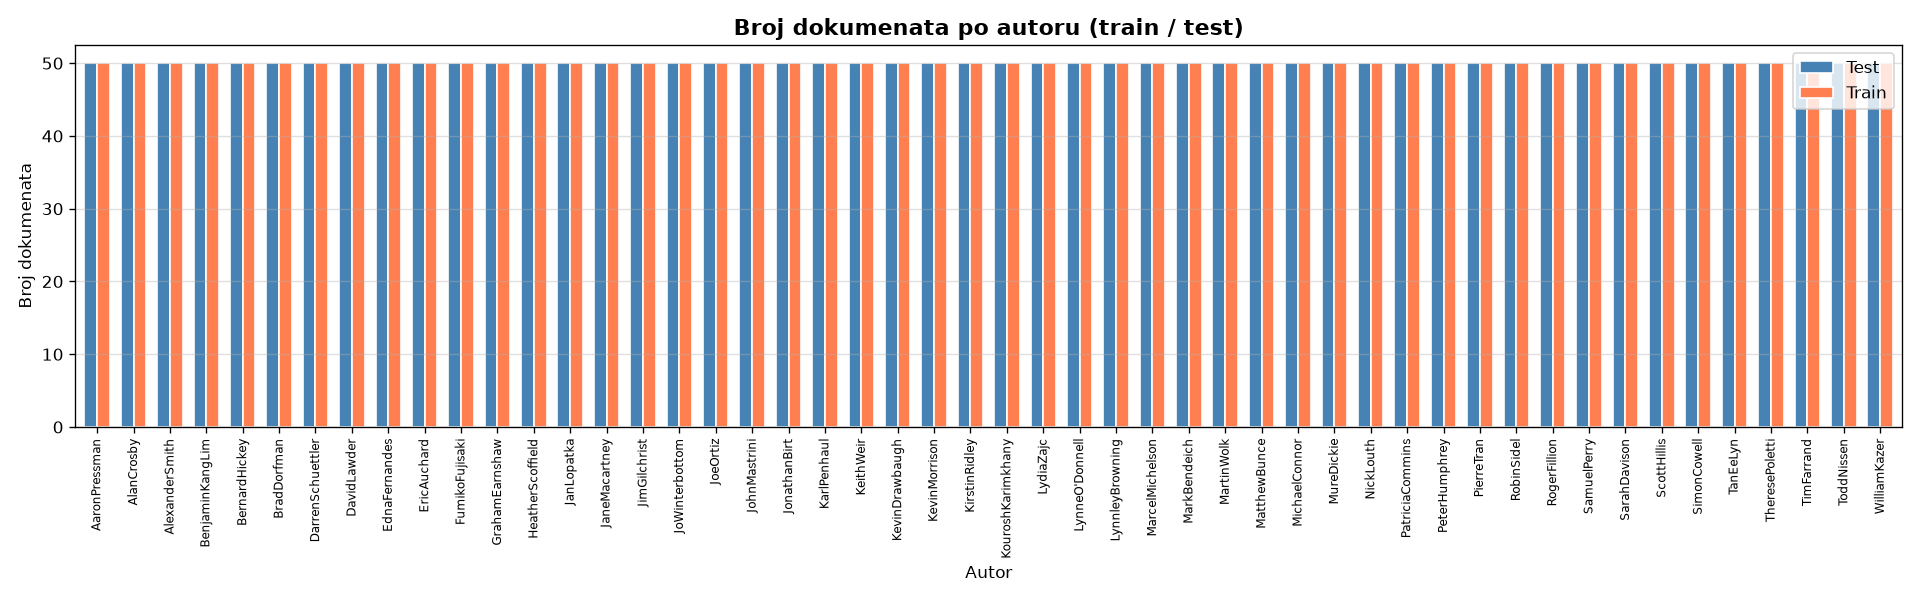
\includegraphics[width=\textwidth]{01_distribucija_autora.png}
        \caption{Broj dokumenata po autoru (train/test)}
    \end{subfigure}
    \hfill
    \begin{subfigure}[b]{0.48\textwidth}
        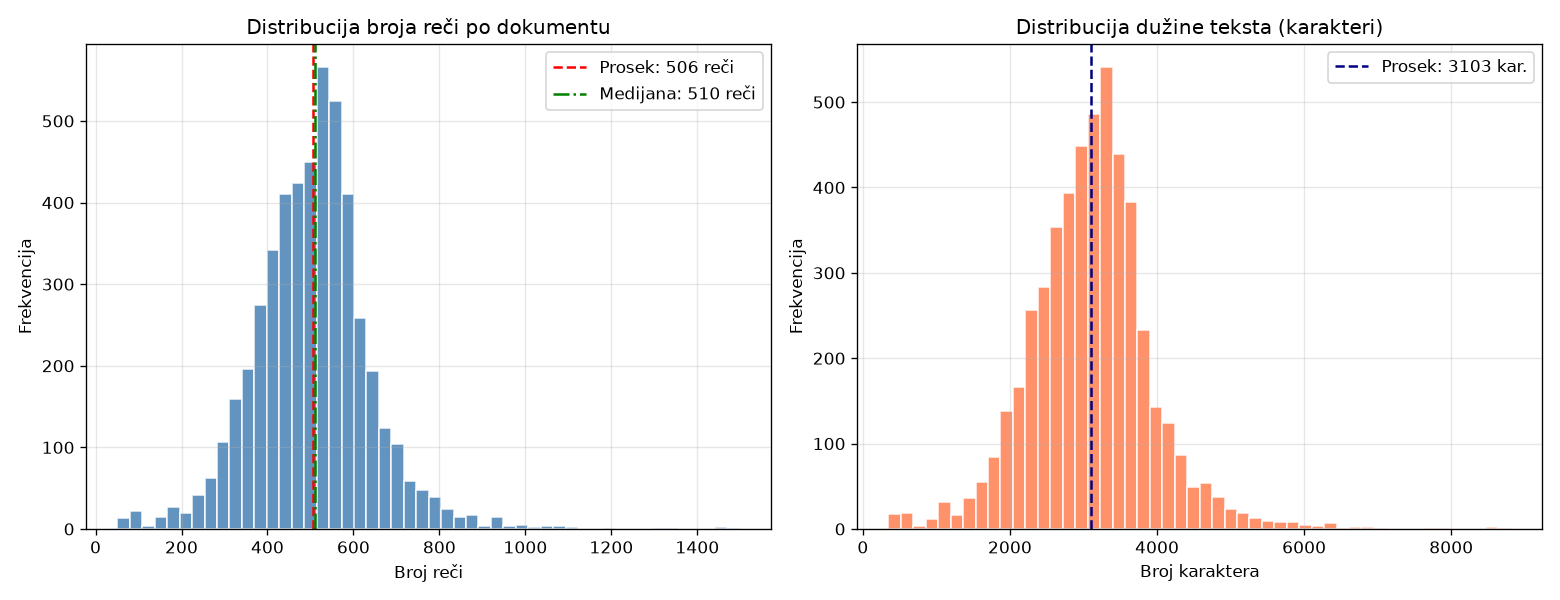
\includegraphics[width=\textwidth]{02_distribucija_duzine.png}
        \caption{Distribucija dužine tekstova}
    \end{subfigure}
    \caption{Osnovna eksploracija Reuters C50 dataseta}
    \label{fig:eksploracija}
\end{figure}

Grafikon \ref{fig:eksploracija}a potvrđuje savršenu balansiranost dataseta — svaki
autor ima tačno 50 train i 50 test dokumenata. Grafikon \ref{fig:eksploracija}b
prikazuje distribuciju broja reči (levo) i karaktera (desno) koja je bliska normalnoj
sa blagom pozitivnom asimetrijom.

\begin{figure}[H]
    \centering
    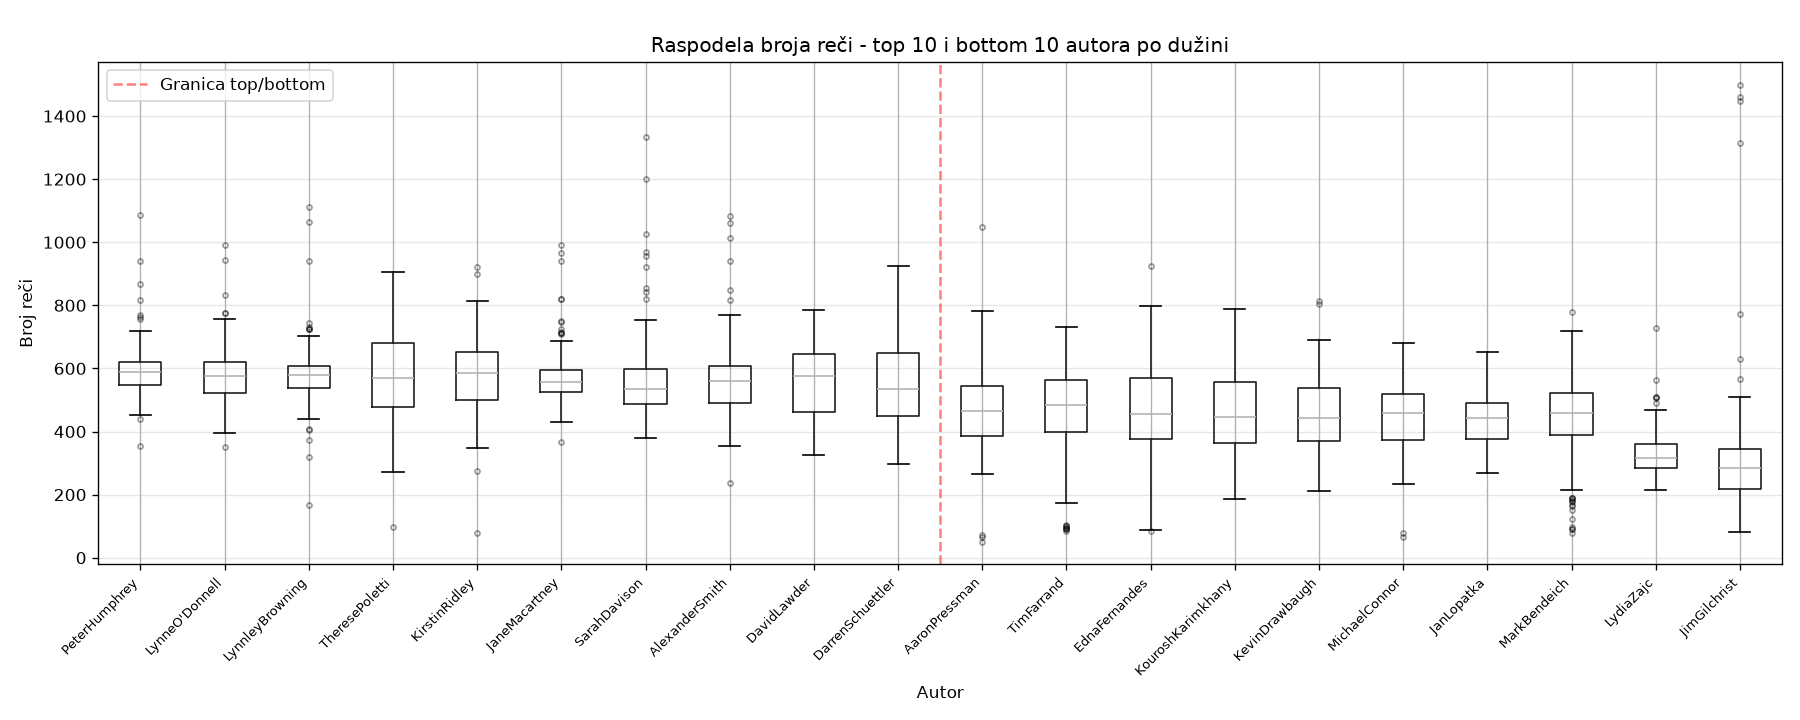
\includegraphics[width=0.85\textwidth]{03_boxplot_duzine.png}
    \caption{Raspodela broja reči — 10 autora s najdužim i 10 s najkraćim tekstovima}
    \label{fig:boxplot}
\end{figure}

Boxplot na slici \ref{fig:boxplot} otkriva da autori s dugačkim tekstovima
(PeterHumphrey, LynneO'Donnell) imaju i veću varijabilnost u dužini, dok autori kratkih
tekstova pišu konzistentno.

% ============================================================
%  3. PREPROCESIRANJE PODATAKA
% ============================================================
\section{Preprocesiranje podataka}

\subsection{Koraci preprocesiranja}

Sirovi novinski tekstovi sadrže šum koji otežava klasifikaciju: HTML/XML tagove,
interpunkciju, brojeve, gramatičke reči bez semantičke vrednosti i varijante iste reči
u različitim morfološkim oblicima. Primenjeni su sledeći koraci preprocesiranja:

\begin{enumerate}
    \item \textbf{Uklanjanje HTML/XML tagova} — regularnim izrazom \texttt{<[{\textasciicircum}>]+>}
    \item \textbf{Filtriranje znakova} — zadržavaju se samo slova i razmaci
    \item \textbf{Lowercase normalizacija} — svi tokeni se pretvaraju u mala slova
    \item \textbf{Tokenizacija} — deljenje teksta na reči
    \item \textbf{Uklanjanje stop-reči} — standardne engleske stop-reči (NLTK) + domenske
    \item \textbf{Filtriranje kratkih tokena} — uklanjaju se reči kraće od 3 karaktera
    \item \textbf{Stemovanje (Porter Stemmer)} — svođenje reči na koren oblika
\end{enumerate}

\subsection{Domenske stop-reči}

Pored standardnih engleskih stop-reči, dodato je i 24 domenske stop-reči specifičnih
za Reuters novinske tekstove:

\begin{center}
\texttt{reuters, said, say, says, year, years, new, also, would, could, may, one, two, three,
inc, corp, lt, dlrs, mln, bln, pct, vs, told, added}
\end{center}

Reči poput \textit{said} i \textit{reuters} pojavljuju se u skoro svakom tekstu i ne
doprinose razlikovanju autora.

\subsection{Efekat preprocesiranja}

\begin{table}[H]
\centering
\caption{Efekat preprocesiranja na broj reči}
\begin{tabular}{lrrr}
\toprule
\textbf{Metrika}    & \textbf{Pre}  & \textbf{Posle} & \textbf{Smanjenje} \\
\midrule
Prosečan broj reči  & 505.7         & 275.8          & 45.5\%             \\
Std. devijacija     & 135.5         & 74.8           & 44.8\%             \\
Minimum             & 51            & 31             & ---                \\
Medijana            & 510           & 276            & 45.9\%             \\
Maksimum            & 1499          & 797            & ---                \\
\bottomrule
\end{tabular}
\end{table}

Preprocesiranje je smanjilo prosečan broj reči za \textbf{45.5\%} — gotovo polovina
svih reči su bile stop-reči, interpunkcija i brojevi bez semantičke vrednosti.
Distribucija ostaje simetrična (prosek $\approx$ medijana = 276 reči).

\begin{figure}[H]
    \centering
    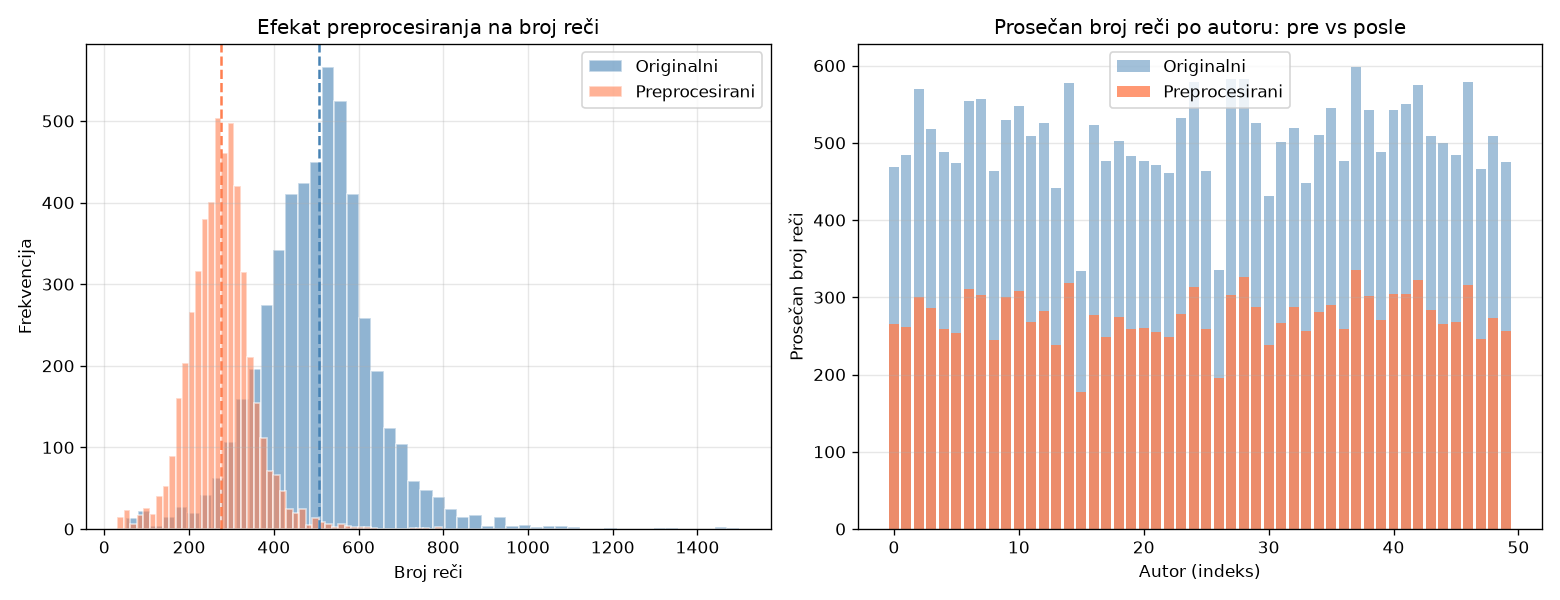
\includegraphics[width=\textwidth]{04_efekat_preprocesiranja.png}
    \caption{Vizualizacija efekta preprocesiranja na broj reči po dokumentu i autoru}
    \label{fig:preprocesiranje}
\end{figure}

\begin{figure}[H]
    \centering
    \begin{subfigure}[b]{0.48\textwidth}
        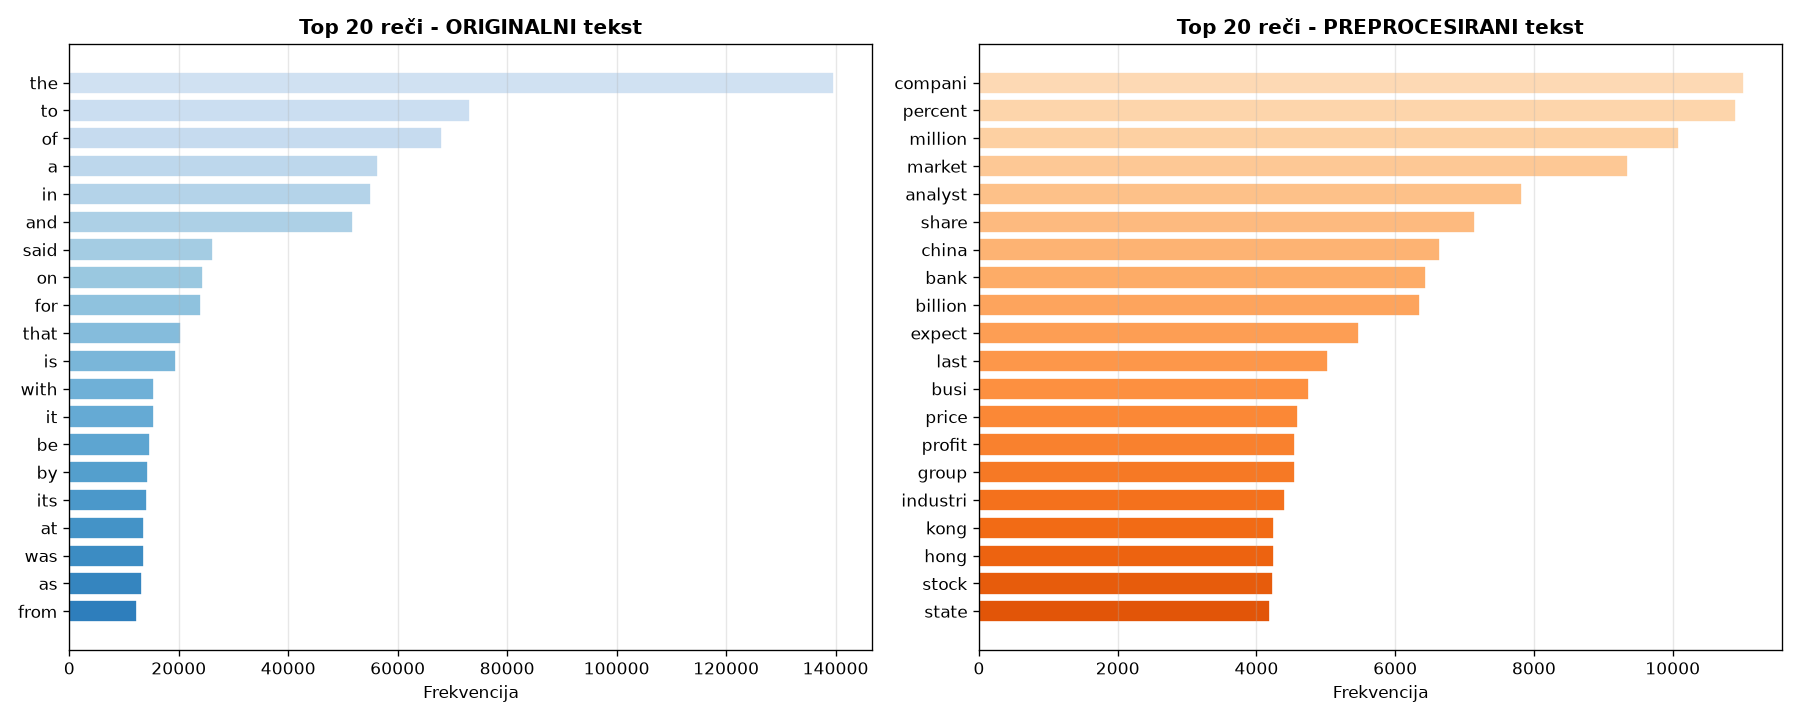
\includegraphics[width=\textwidth]{05_top20_reci_pre_posle.png}
        \caption{Top 20 reči pre i posle preprocesiranja}
    \end{subfigure}
    \hfill
    \begin{subfigure}[b]{0.48\textwidth}
        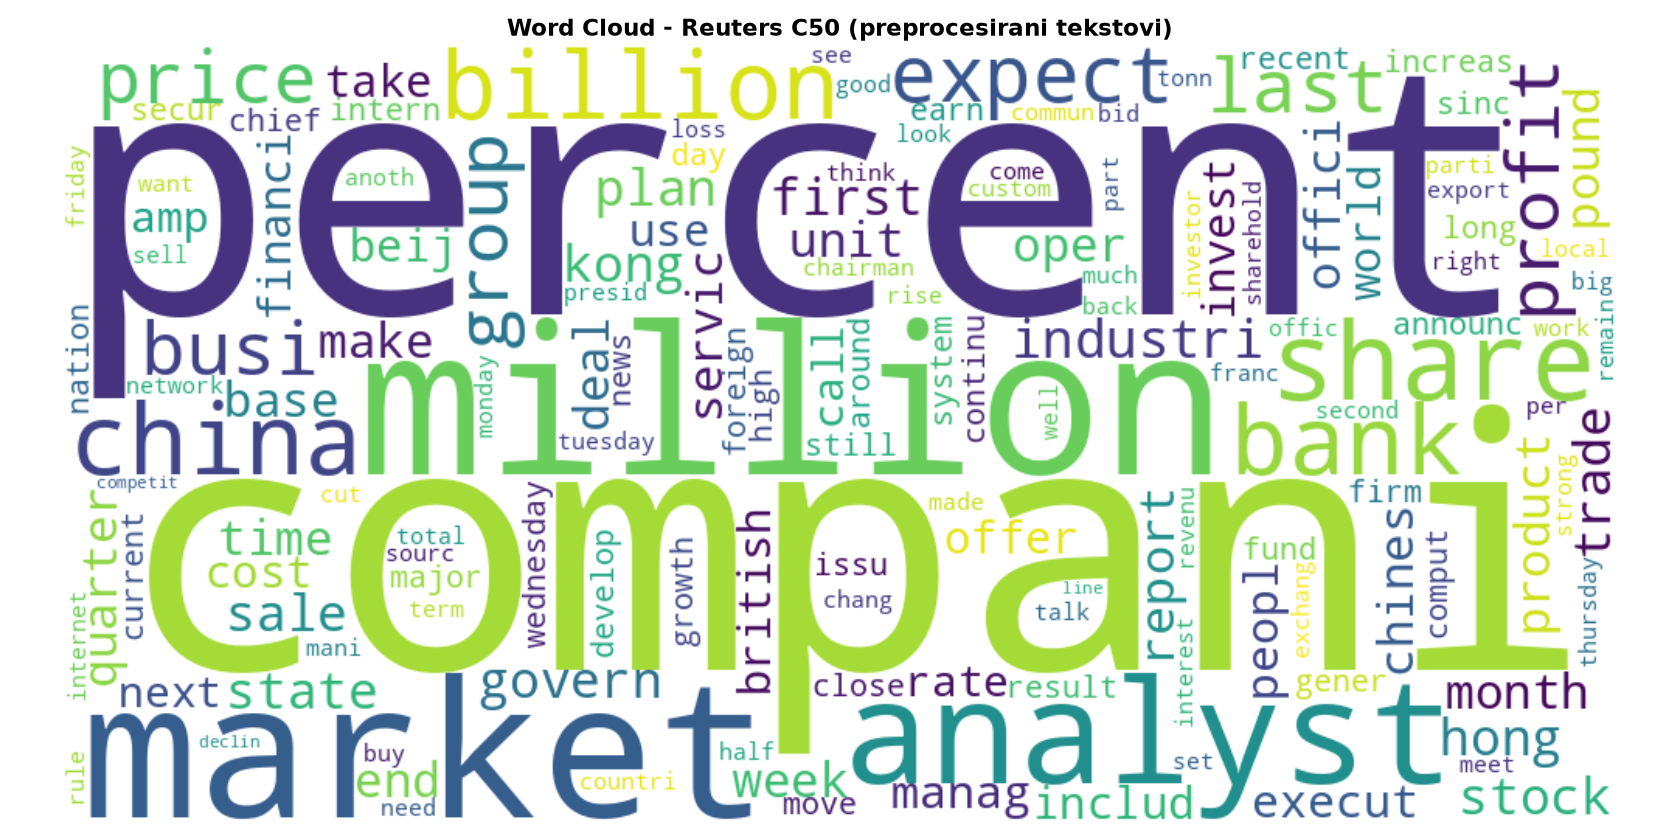
\includegraphics[width=\textwidth]{06_wordcloud.png}
        \caption{Word Cloud (preprocesirani tekstovi)}
    \end{subfigure}
    \caption{Analiza frekvencije reči}
    \label{fig:reci}
\end{figure}

Pre preprocesiranja, top 20 reči su isključivo gramatičke stop-reči
(\textit{the, to, of, a, in, and, said...}). Nakon preprocesiranja, top reči su
smisleni finansijski termini: \textbf{compani, percent, million, market, analyst,
share, china, bank, billion} — što odgovara tematici Reuters agencije.
Prisustvo reči \textit{china, hong, kong} ukazuje na značajnu pokrivenost
azijskog tržišta.

% ============================================================
%  4. VIZUALIZACIJA U 2D I 3D PROSTORU
% ============================================================
\section{Vizualizacija podataka u 2D i 3D prostoru}

\subsection{TF-IDF vektorizacija za vizualizaciju}

Pošto tekstualni podaci nemaju direktnu prostornu reprezentaciju, koristimo
tehnike redukcije dimenzionalnosti za vizualizaciju. TF-IDF matricu dimenzija
$5000 \times 5000$ (96.8\% nula) nije moguće direktno vizualizovati, pa je
primenjena sledeća pipeline:

\[
\text{Tekst} \xrightarrow{\text{TF-IDF}} \mathbb{R}^{5000} \xrightarrow{\text{SVD}} \mathbb{R}^{100} \xrightarrow{\text{PCA/t-SNE}} \mathbb{R}^{2/3}
\]

\subsection{SVD redukcija dimenzionalnosti}

TruncatedSVD je primenjen kao predkorak koji radi direktno na retkim matricama.

\begin{figure}[H]
    \centering
    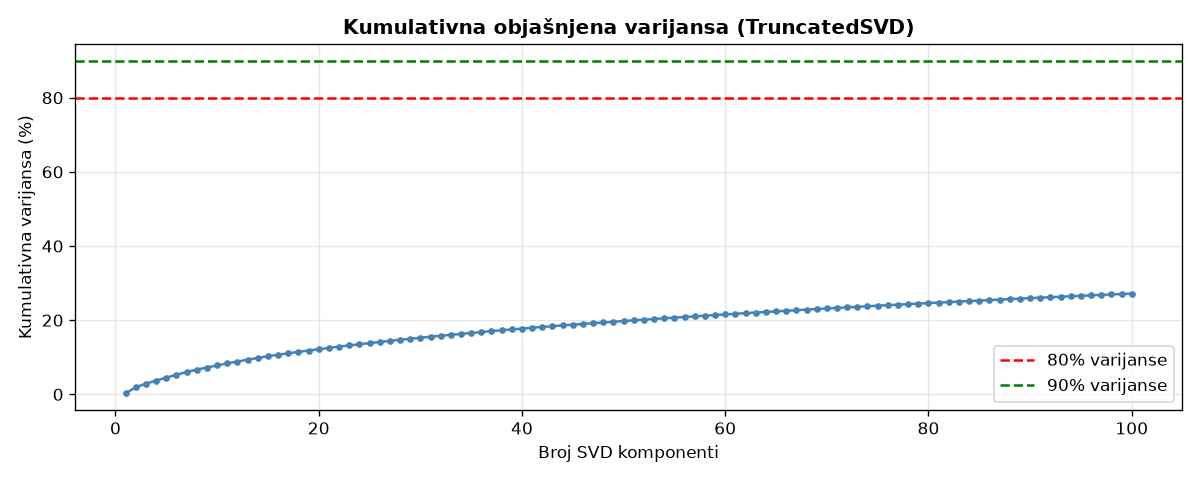
\includegraphics[width=0.8\textwidth]{07_svd_scree.png}
    \caption{Scree plot — kumulativna objašnjena varijansa (TruncatedSVD, 100 komponenti)}
    \label{fig:scree}
\end{figure}

Sa 100 SVD komponenti objašnjava se samo \textbf{27.2\%} ukupne varijanse.
Kriva raste postepeno bez strme „laktične" tačke, što je karakteristično za
visoko-dimenzionalne tekstualne podatke — informacija je ravnomerno rasuta
po svim dimenzijama i ne može se efikasno kompresovati.

\subsection{PCA vizualizacija}

\begin{figure}[H]
    \centering
    \begin{subfigure}[b]{0.55\textwidth}
        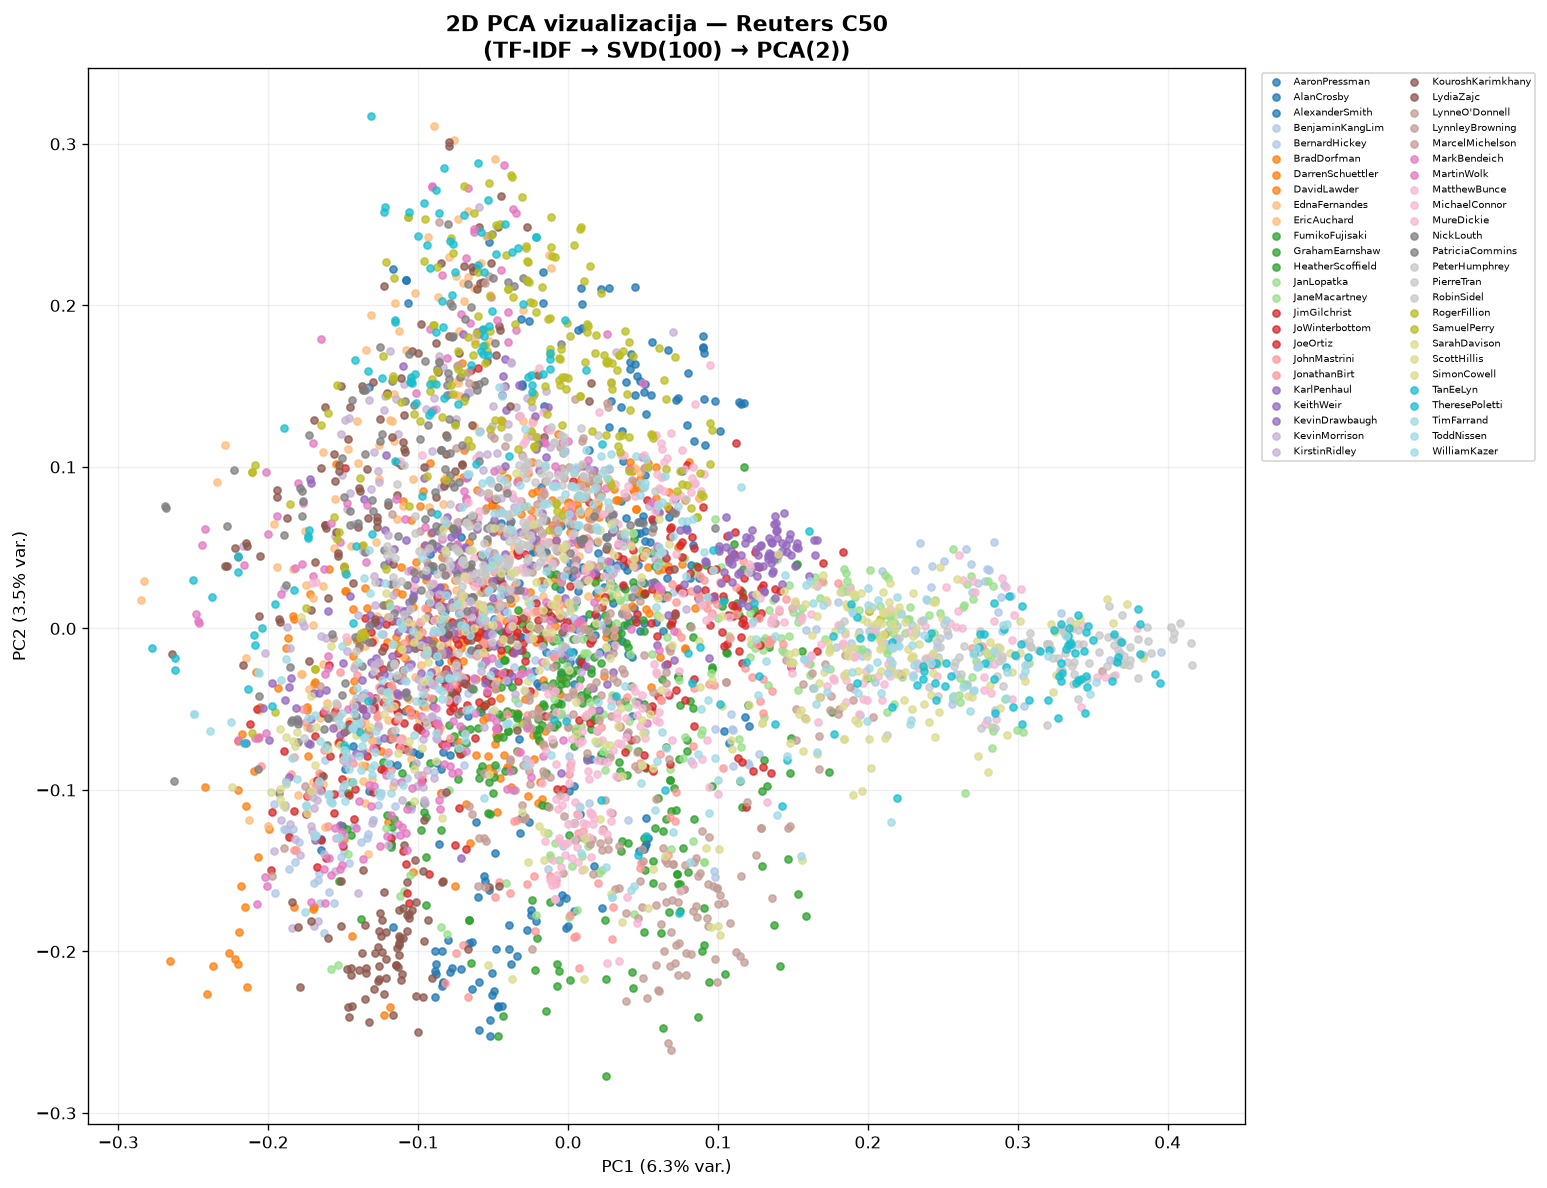
\includegraphics[width=\textwidth]{08_pca_2d.png}
        \caption{PCA 2D projekcija (PC1=6.30\%, PC2=3.53\%)}
    \end{subfigure}
    \hfill
    \begin{subfigure}[b]{0.42\textwidth}
        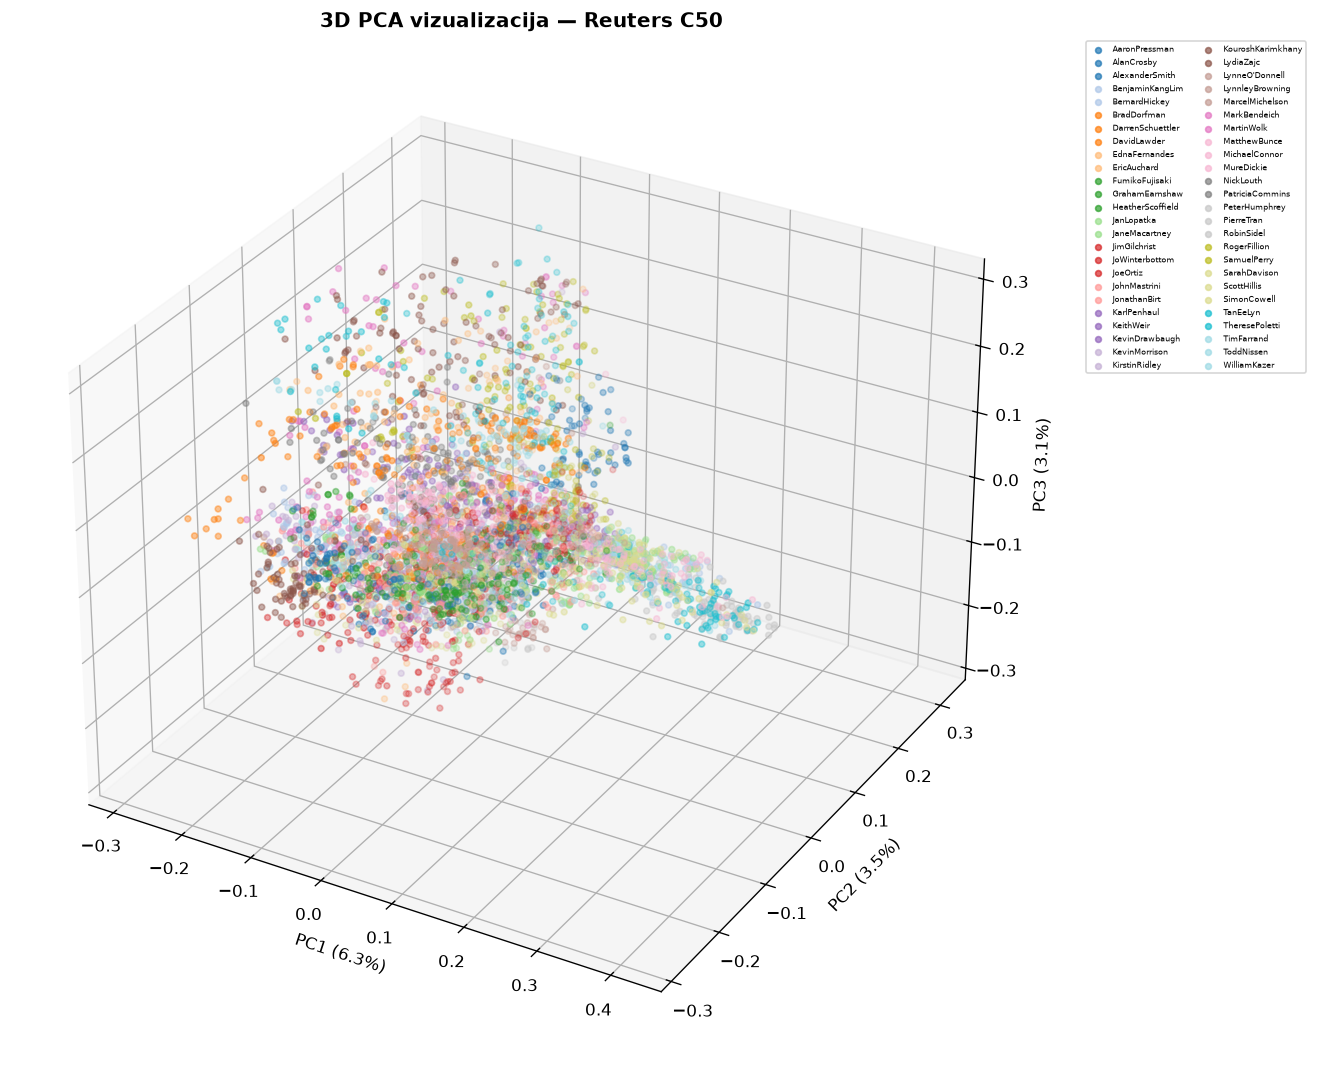
\includegraphics[width=\textwidth]{09_pca_3d.png}
        \caption{PCA 3D projekcija (ukupno 12.94\%)}
    \end{subfigure}
    \caption{PCA vizualizacija svih 5000 dokumenata obojenih po autoru}
    \label{fig:pca}
\end{figure}

PC1 objašnjava 6.30\%, a PC2 3.53\% varijanse — zajedno svega 9.83\%.
Linearna PCA nije dovoljno moćna da razdvoji 50 autorskih stilova na osnovu
samo 2–3 dimenzije, pa projekcija prikazuje značajno preklapanje klasa.
Ipak, određeni autori su vidljivi kao odvojeni oblaci na rubovima prostora
— oni imaju najdistinktivniji vokabular.

\subsection{t-SNE vizualizacija}

\begin{figure}[H]
    \centering
    \begin{subfigure}[b]{0.55\textwidth}
        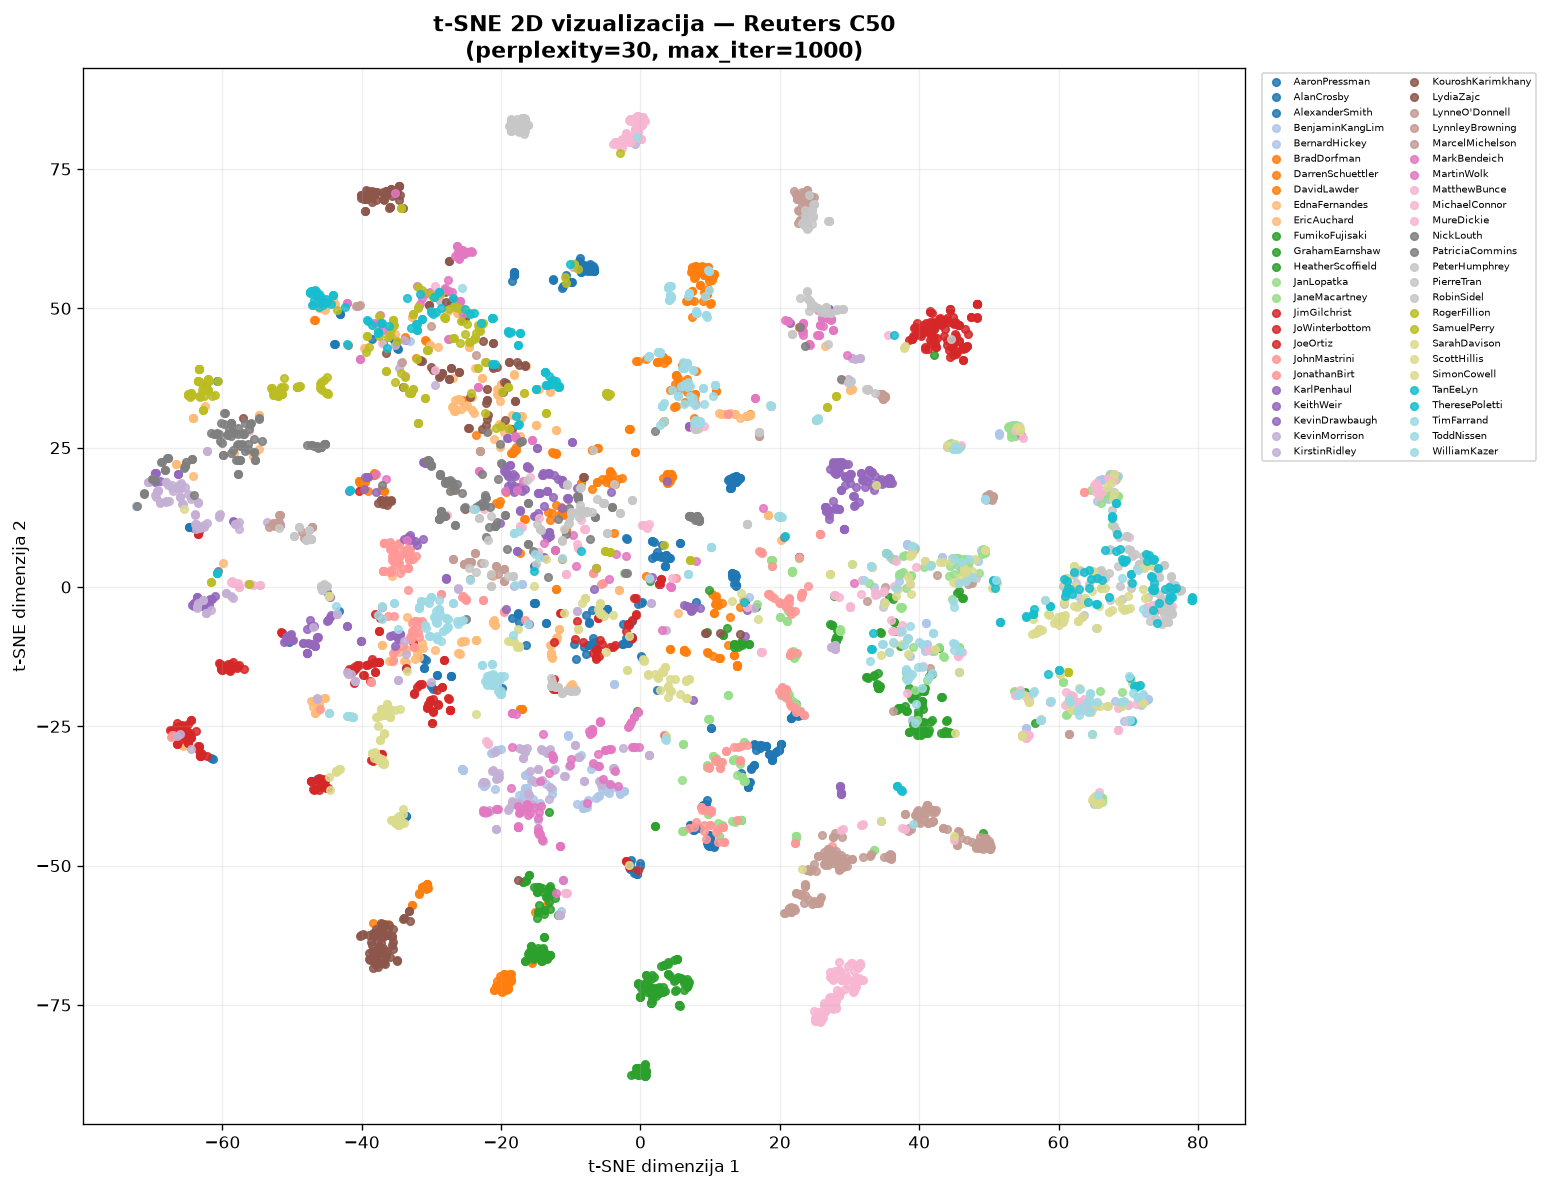
\includegraphics[width=\textwidth]{10_tsne_2d.png}
        \caption{t-SNE 2D (perplexity=30, max\_iter=1000)}
    \end{subfigure}
    \hfill
    \begin{subfigure}[b]{0.42\textwidth}
        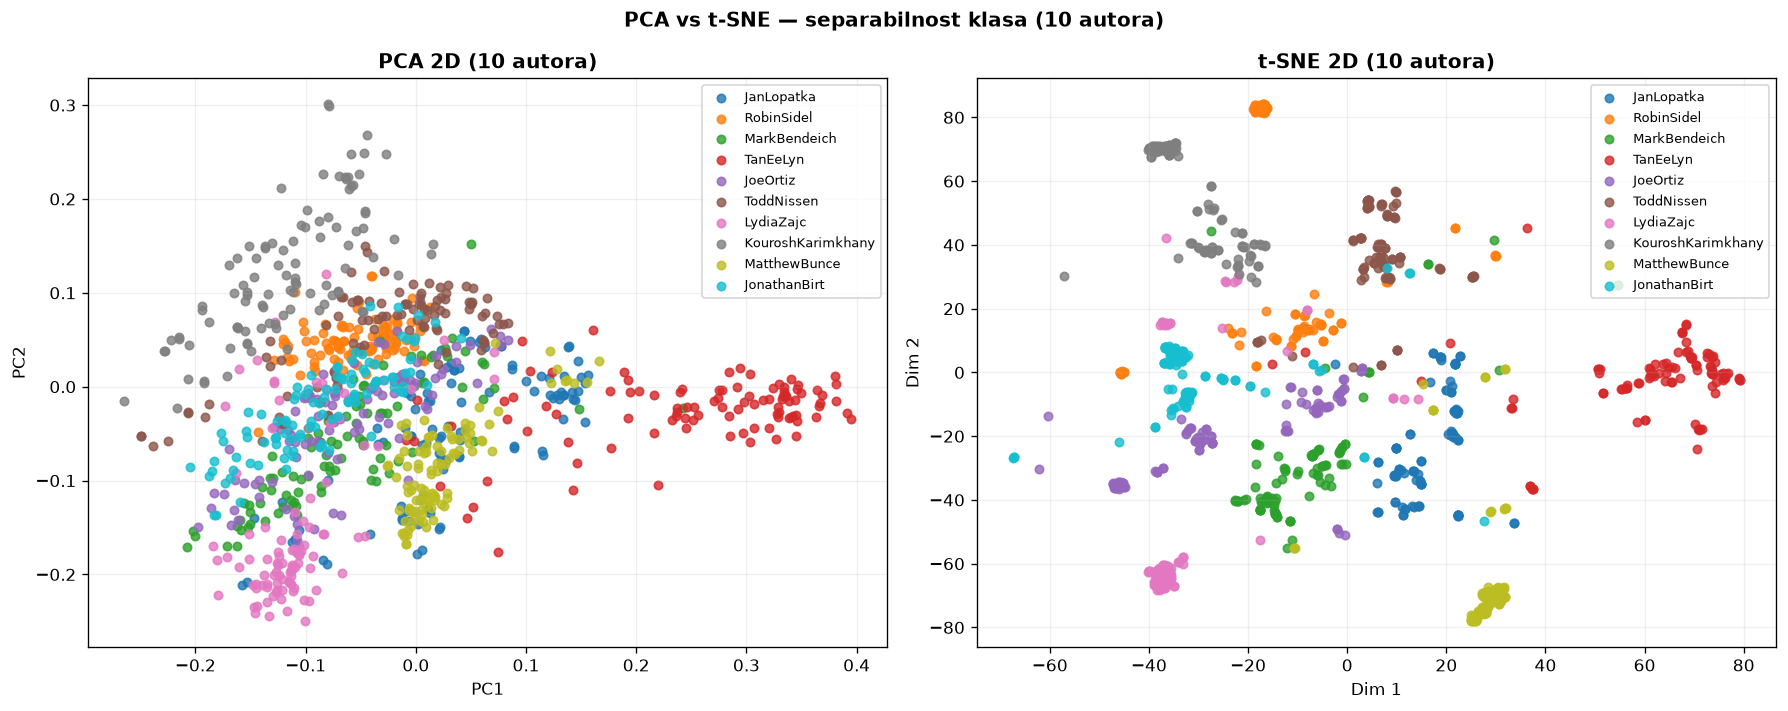
\includegraphics[width=\textwidth]{11_pca_vs_tsne.png}
        \caption{PCA vs t-SNE — 10 nasumičnih autora}
    \end{subfigure}
    \caption{t-SNE vizualizacija i poređenje sa PCA}
    \label{fig:tsne}
\end{figure}

t-SNE, kao nelinearna metoda koja čuva lokalne susedstvene odnose,
pokazuje znatno bolju separaciju klasa od PCA. Vidljivi su kompaktni
klasteri za deo autora, posebno one sa distinktivnim temama (novinari
specijalizovani za jednu geografsku oblast ili temu).

Poređenje na 10 autora (desna slika) jasno ilustruje prednost t-SNE:
dok PCA prikazuje isprepletane oblake tačaka, t-SNE ih razdvaja u
prostorno odvojene grupe. Ovo vizuelno potvrđuje da su autorski stilovi
dovoljno distinktivni da ih algoritmi klasifikacije mogu razlikovati
u punom dimenzionalnom prostoru.

% ============================================================
%  5. TF-IDF VEKTORIZACIJA I KLASIFIKACIJA
% ============================================================
\section{TF-IDF vektorizacija i klasifikacija}

\subsection{TF-IDF vektorizacija}

Za klasifikaciju su kreirana tri TF-IDF skupa atributa različite granularnosti:

\begin{table}[H]
\centering
\caption{Konfiguracije TF-IDF skupova atributa}
\begin{tabular}{llll}
\toprule
\textbf{Naziv}        & \textbf{N-grami}     & \textbf{Max features} & \textbf{Dimenzije} \\
\midrule
Puni skup             & unigrami + bigrami   & 10 000 & $2500 \times 10000$ \\
Redukovani skup       & unigrami             & 2 000  & $2500 \times 2000$  \\
Mali skup             & unigrami             & 500    & $2500 \times 500$   \\
\bottomrule
\end{tabular}
\end{table}

Svi TF-IDF vektorizatori su fitovani \textbf{isključivo na train skupu}, a zatim
primenjeni (\textit{transform}) na test skup — čime se sprečava curenje informacija
(\textit{data leakage}). Korišćeno je sublinearno TF skaliranje ($\text{tf} \to 1 + \log(\text{tf})$)
koje smanjuje uticaj ekstremno čestih reči.

\subsection{Klasifikacioni algoritmi}

Primenjeno je 7 algoritama koji pokrivaju različite pristupe mašinskom učenju:

\begin{table}[H]
\centering
\caption{Primenjeni klasifikacioni algoritmi i njihove konfiguracije}
\begin{tabular}{lll}
\toprule
\textbf{Algoritam}            & \textbf{Pristup}        & \textbf{Ključni hiperparametri} \\
\midrule
Naive Bayes (Multinomial)     & Probabilistički         & $\alpha = 0.1$ \\
Naive Bayes (Complement)      & Probabilistički         & $\alpha = 0.1$ \\
SVM (LinearSVC)               & Linearni diskriminativni & $C = 1.0$ \\
Logistic Regression           & Linearni diskriminativni & $C = 5.0$, solver=lbfgs \\
Random Forest                 & Ansamblski              & 200 stabala \\
K-Nearest Neighbors           & Baziran na instancama   & $k=5$, metrika: kosinusna \\
Decision Tree                 & Stabla odluke           & max\_depth=50 \\
\bottomrule
\end{tabular}
\end{table}

KNN koristi \textbf{kosinusnu metriku} koja je prikladnija za TF-IDF vektore od
euklidske — bolje hvata ugaonu sličnost između dokumenata u visokim dimenzijama.

% ============================================================
%  6. REZULTATI KLASIFIKACIJE
% ============================================================
\section{Rezultati klasifikacije}

\subsection{Accuracy po algoritmu i skupu atributa}

\begin{table}[H]
\centering
\caption{Accuracy (\%) svih 21 modela}
\setlength{\tabcolsep}{8pt}
\begin{tabular}{lccc}
\toprule
\textbf{Klasifikator} & \textbf{Mali (500)} & \textbf{Redukovani (2000)} & \textbf{Puni (10000)} \\
\midrule
\rowcolor{rowgray}
SVM (LinearSVC)           & 66.28 & 70.88 & \textbf{72.40} \\
Logistic Regression       & 66.88 & 70.36 & 71.04 \\
\rowcolor{rowgray}
Naive Bayes (Multinomial) & 60.72 & 65.44 & 67.52 \\
Random Forest             & 60.00 & 63.84 & 66.20 \\
\rowcolor{rowgray}
Naive Bayes (Complement)  & 51.16 & 59.20 & 63.76 \\
K-Nearest Neighbors       & 55.36 & 58.72 & 60.92 \\
\rowcolor{rowgray}
Decision Tree             & 38.16 & 43.84 & 45.28 \\
\bottomrule
\end{tabular}
\end{table}

\begin{figure}[H]
    \centering
    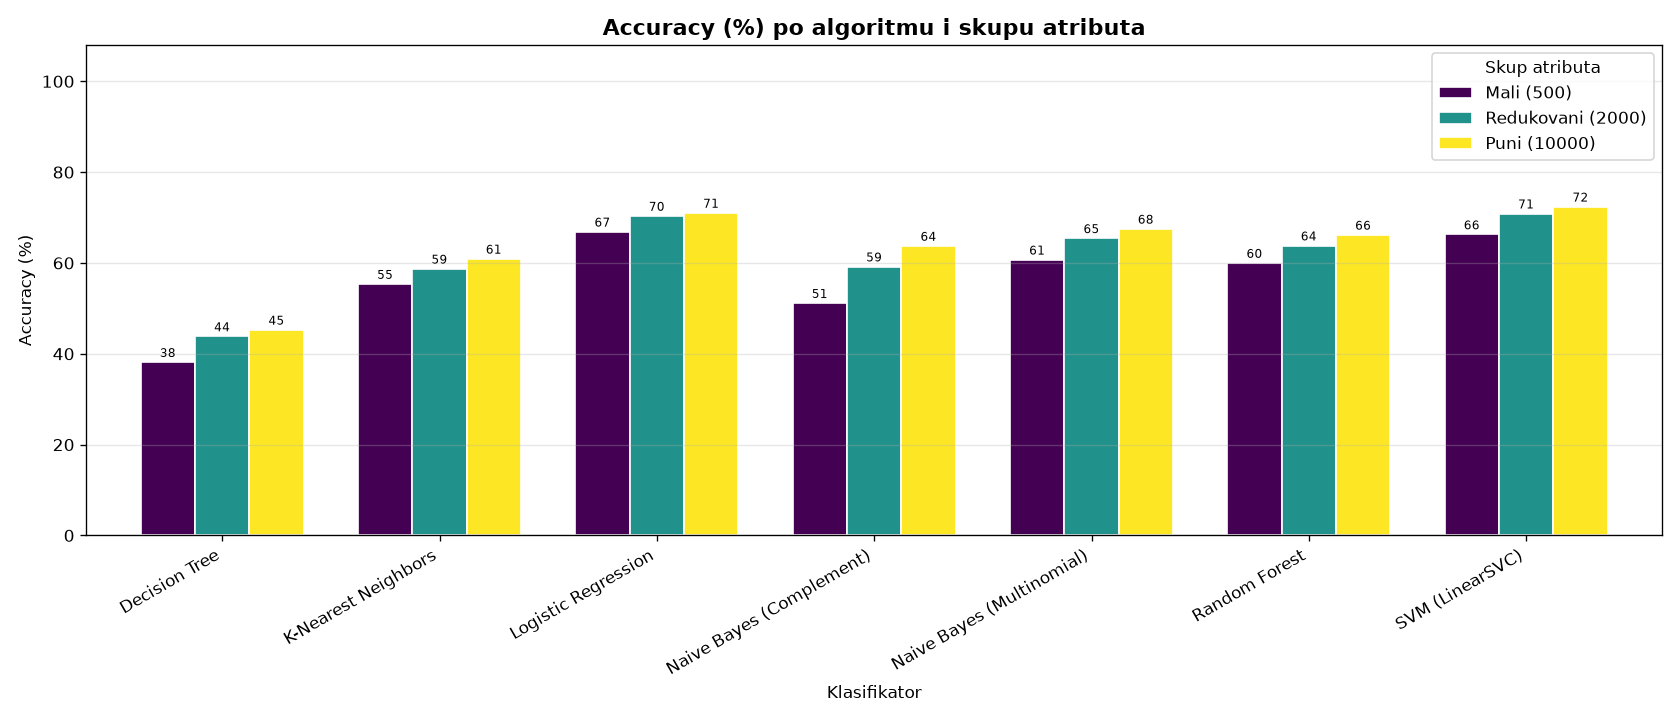
\includegraphics[width=\textwidth]{12_accuracy_bar.png}
    \caption{Accuracy (\%) po algoritmu i skupu atributa — grouped bar chart}
    \label{fig:accuracy_bar}
\end{figure}

\subsection{Analiza rezultata}

Iz rezultata se mogu izvući sledeći zaključci:

\begin{enumerate}
    \item \textbf{SVM (LinearSVC)} je globalno najbolji model sa \textbf{72.40\% tačnosti}
    i 72.03\% macro F1 na punom skupu atributa.

    \item \textbf{Logistička regresija} je blizu (71.04\%), što potvrđuje da linearni modeli
    dominiraju u klasifikaciji TF-IDF vektora.

    \item \textbf{Povećanje broja atributa} konzistentno poboljšava sve modele.
    Dobitak od 500 na 2000 je veći nego od 2000 na 10000, što sugeriše zasićivanje krive.

    \item \textbf{Naive Bayes Complement} je najosjetljiviji na redukciju atributa:
    gubi 12.6 pp (63.8\% $\to$ 51.2\%) prelaskom sa punog na mali skup.

    \item \textbf{Decision Tree} je ubedljivo najlošiji (45.3\%) — stabla odluke
    loše generalizuju na retkim visoko-dimenzionalnim TF-IDF matricama.
\end{enumerate}

\begin{figure}[H]
    \centering
    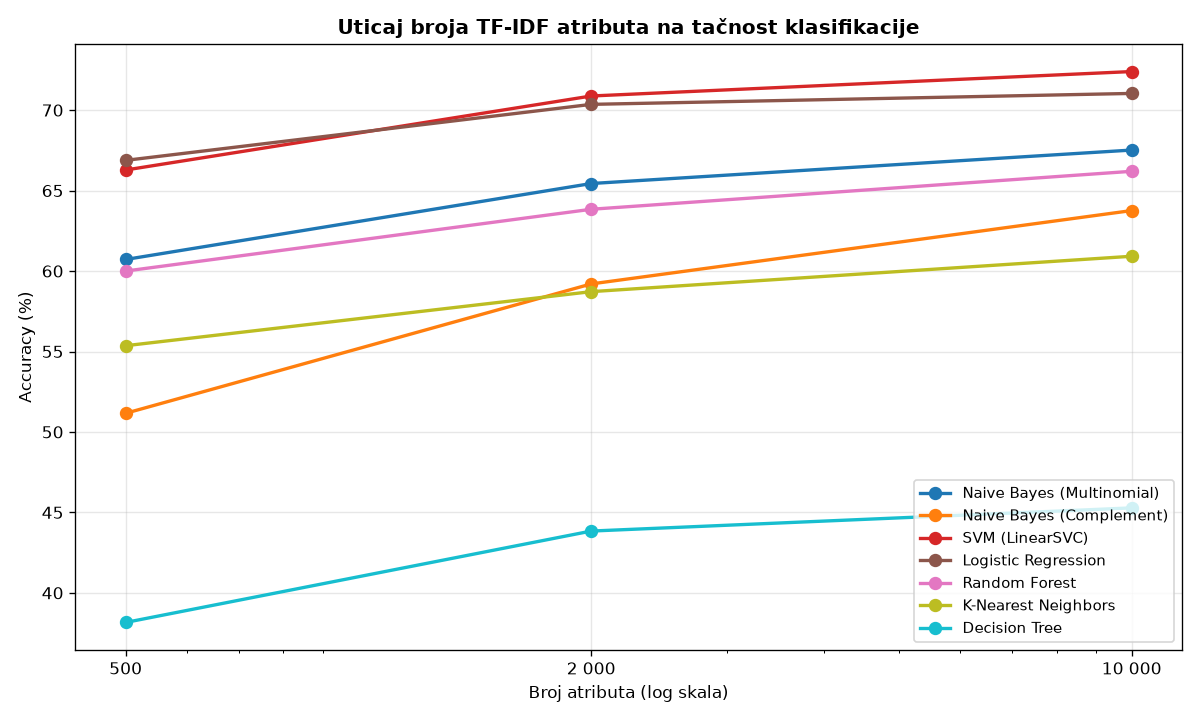
\includegraphics[width=\textwidth]{14_efekat_broja_atributa.png}
    \caption{Uticaj broja TF-IDF atributa na tačnost klasifikacije (log skala)}
    \label{fig:atributi}
\end{figure}

Slika \ref{fig:atributi} jasno prikazuje da su krive SVM i LR najravnije
(najrobusnije na smanjenje atributa), dok Naive Bayes Complement ima najstrmiji pad.

\subsection{Poređenje svih metrika (puni skup atributa)}

\begin{figure}[H]
    \centering
    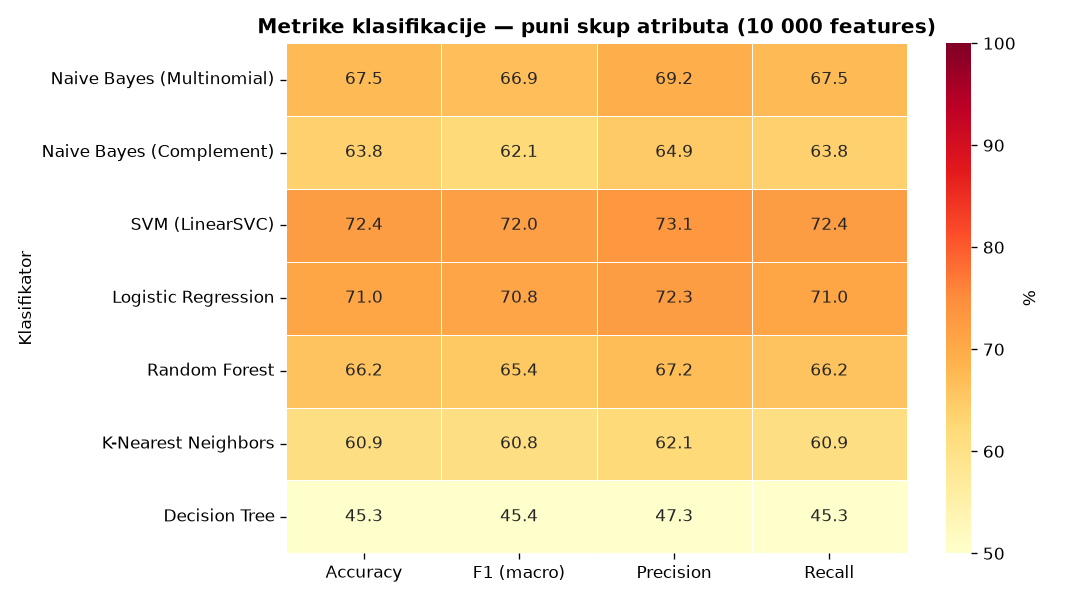
\includegraphics[width=0.85\textwidth]{13_heatmap_metrike.png}
    \caption{Heatmap svih metrika klasifikacije — puni skup atributa (10 000 features)}
    \label{fig:heatmap}
\end{figure}

Heatmap na slici \ref{fig:heatmap} pokazuje da su sve četiri metrike (Accuracy,
F1 macro, Precision, Recall) međusobno konzistentne — razlika između njih je manja
od 1 pp za svaki model. Ovo potvrđuje da je dataset balansiran i da nema dominantnih
klasa koje bi narušavale metrike.

% ============================================================
%  7. DETALJNA EVALUACIJA
% ============================================================
\section{Detaljna evaluacija}

\subsection{Confusion matrica (SVM, puni skup)}

\begin{figure}[H]
    \centering
    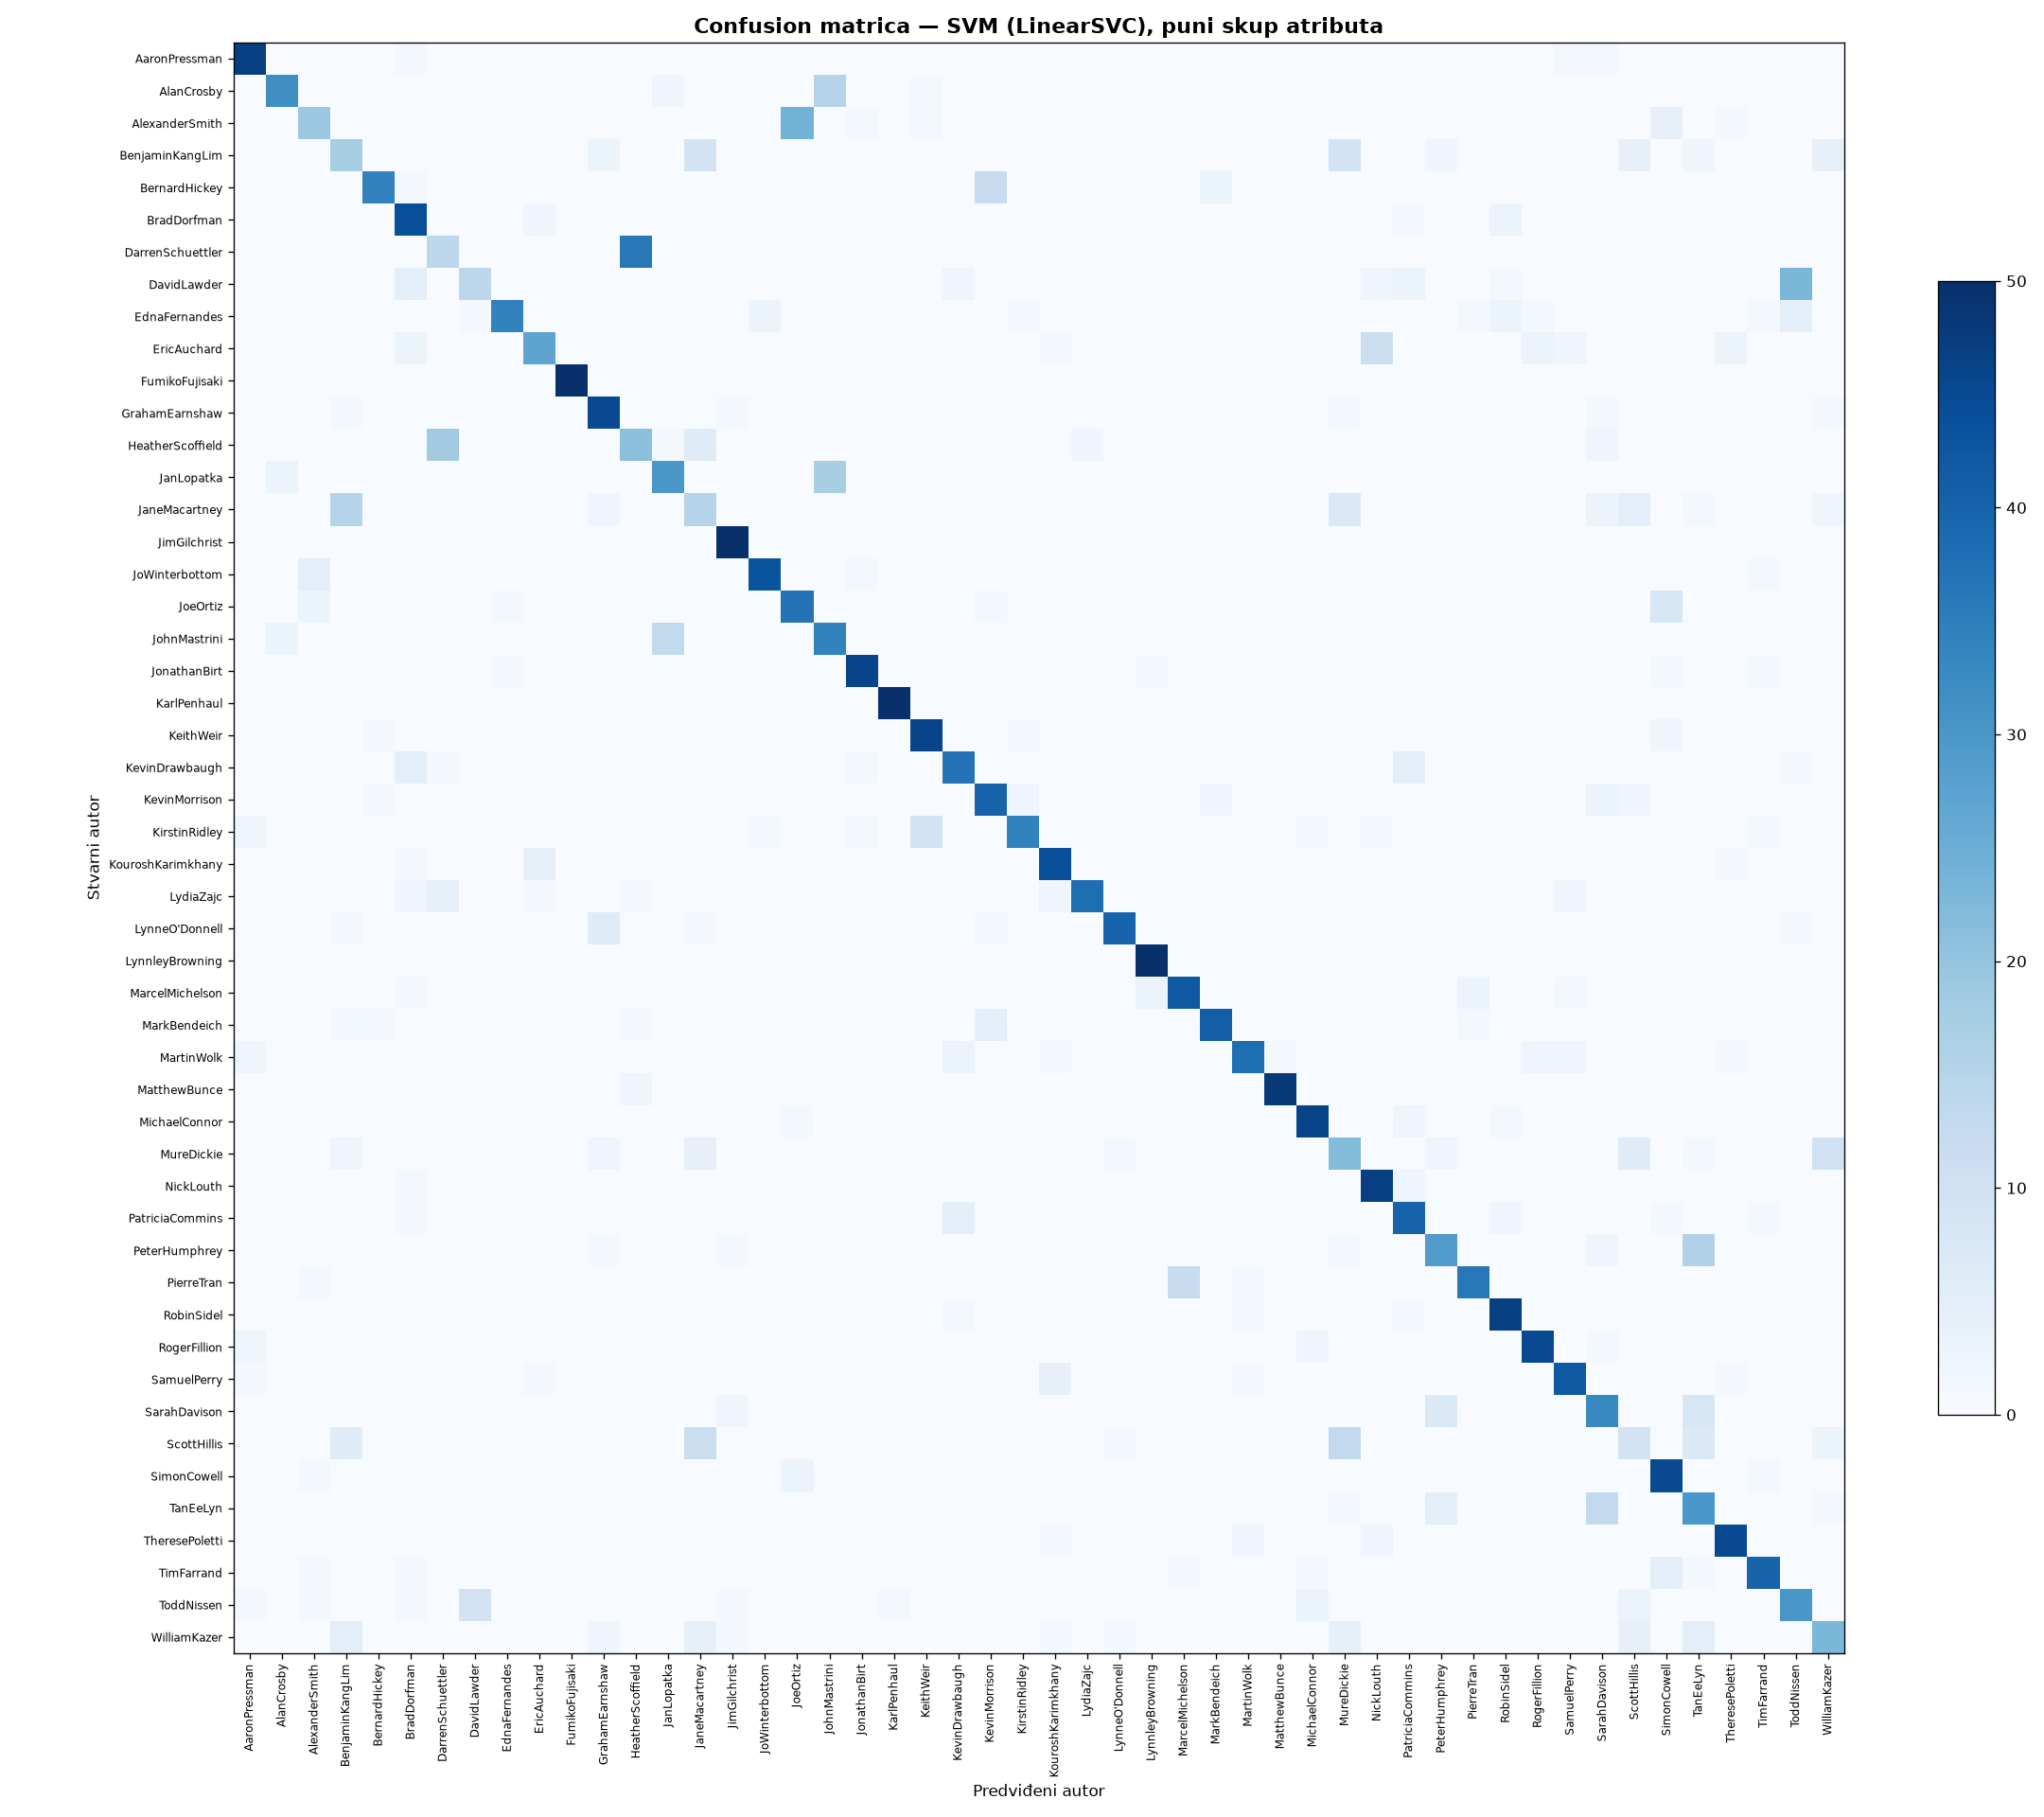
\includegraphics[width=\textwidth]{15_confusion_matrix.png}
    \caption{Confusion matrica — SVM (LinearSVC) na punom skupu atributa}
    \label{fig:confusion}
\end{figure}

Confusion matrica na slici \ref{fig:confusion} vizualizuje distribuciju
tačnih i pogrešnih predikcija za svih 50 autora. Tamno-plavi dijagonalni
elementi označavaju tačne klasifikacije — dominantni su za većinu autora.

Posebno se ističu:
\begin{itemize}
    \item \textbf{Savršeno klasifikovani autori} (100\% recall):
    FumikoFujisaki, JimGilchrist, LynnleyBrowning, KarlPenhaul —
    svi njihovi dokumenti su tačno prepoznati.
    \item \textbf{Najlošije klasifikovani autori}: ScottHillis (18\%),
    DarrenSchuettler i DavidLawder (po 28\%), JaneMacartney (30\%).
\end{itemize}

\subsection{Analiza tačnosti po autorima}

\begin{figure}[H]
    \centering
    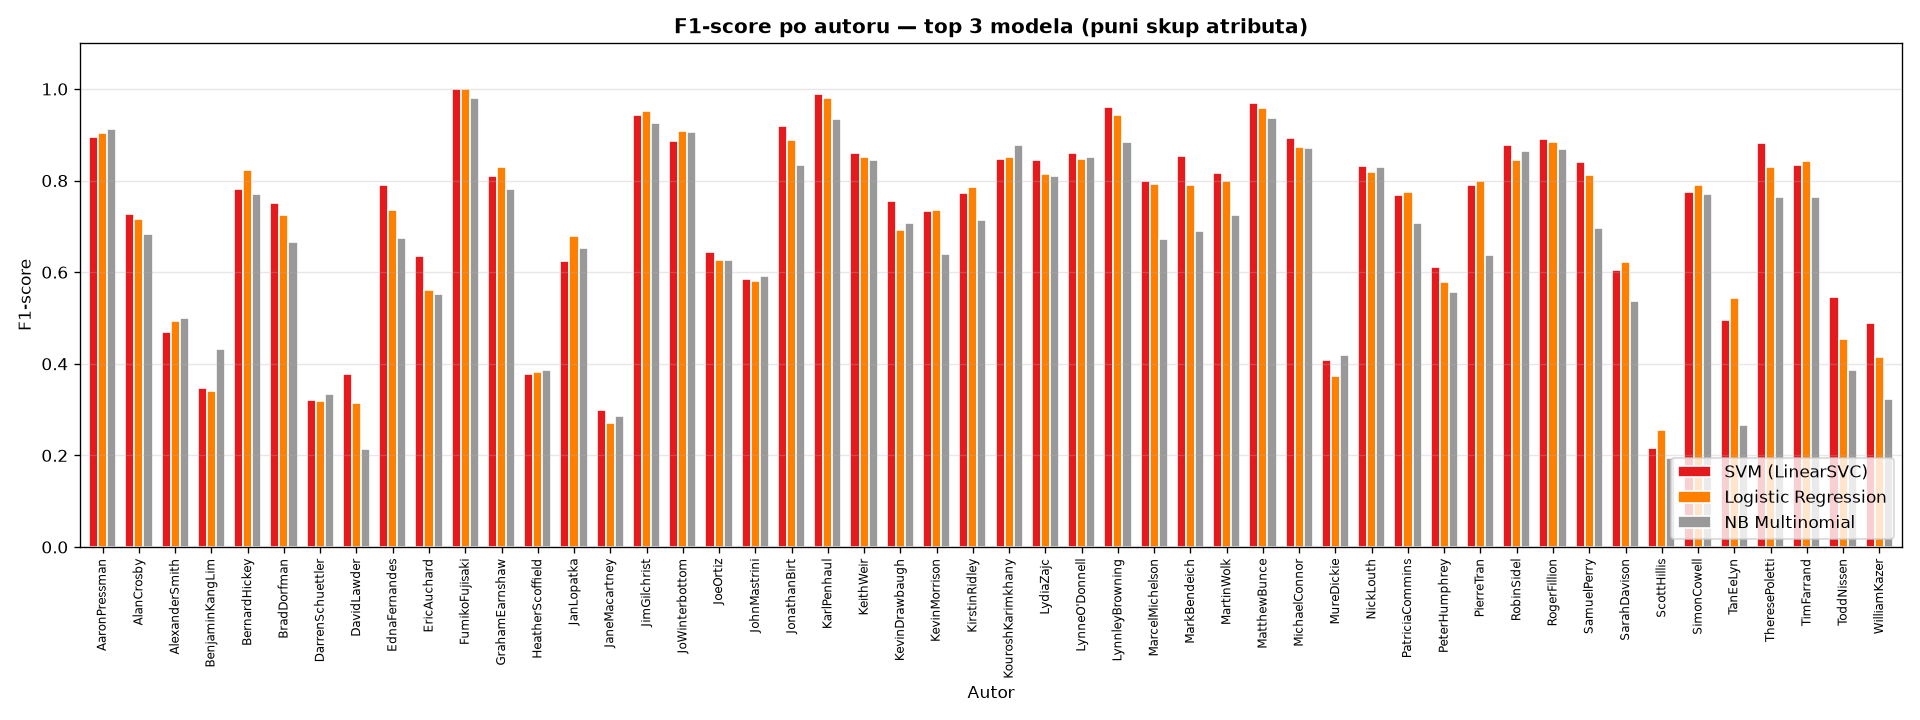
\includegraphics[width=\textwidth]{16_f1_per_author.png}
    \caption{F1-score po autoru za top 3 modela (puni skup atributa)}
    \label{fig:f1_author}
\end{figure}

\begin{figure}[H]
    \centering
    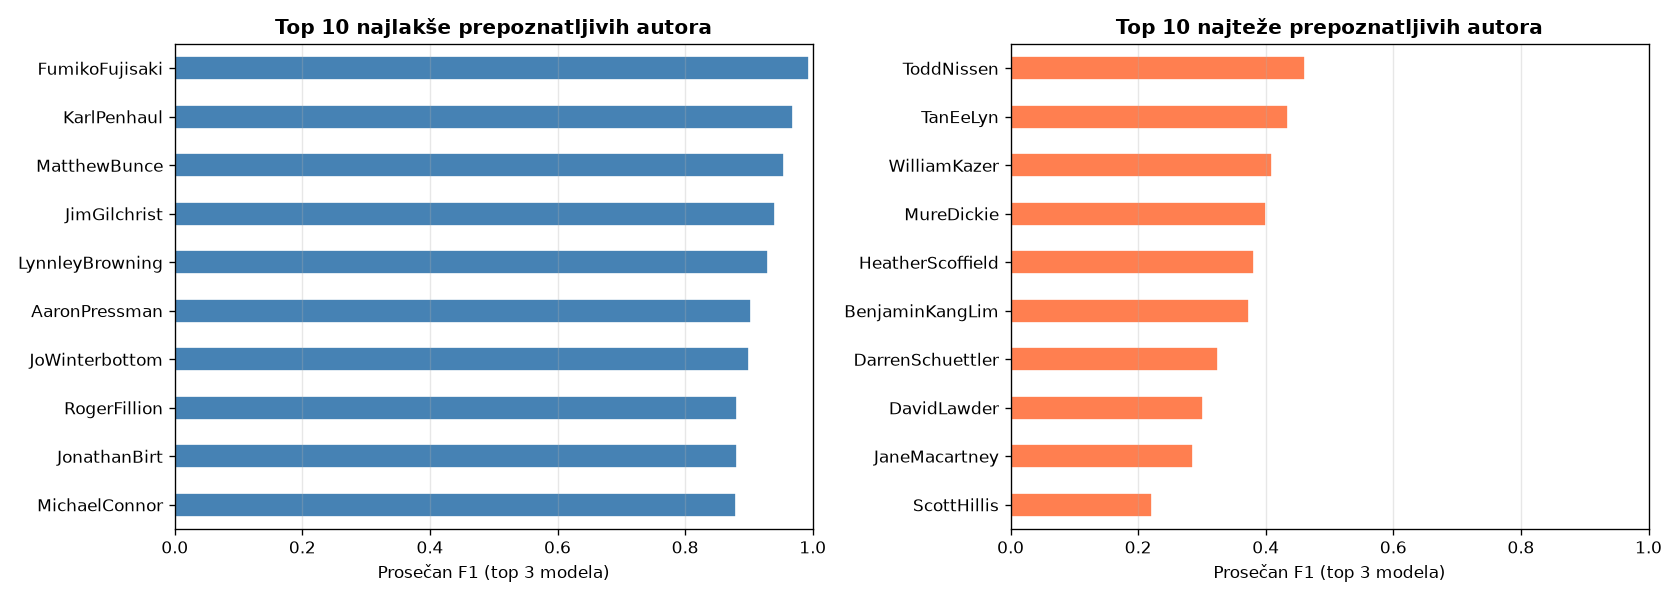
\includegraphics[width=\textwidth]{17_laki_teski_autori.png}
    \caption{Top 10 najlakše i najteže prepoznatljivih autora (prosečan F1 top 3 modela)}
    \label{fig:laki_teski}
\end{figure}

\begin{table}[H]
\centering
\caption{10 najlakše i 10 najteže prepoznatljivih autora (prosečan F1, top 3 modela)}
\begin{tabular}{lc|lc}
\toprule
\multicolumn{2}{c|}{\textbf{Najlakši autori}} & \multicolumn{2}{c}{\textbf{Najteži autori}} \\
\textbf{Autor}         & \textbf{F1} & \textbf{Autor}        & \textbf{F1} \\
\midrule
FumikoFujisaki         & 0.993       & ScottHillis           & 0.222 \\
KarlPenhaul            & 0.968       & JaneMacartney         & 0.286 \\
MatthewBunce           & 0.955       & DavidLawder           & 0.302 \\
JimGilchrist           & 0.941       & DarrenSchuettler      & 0.324 \\
LynnleyBrowning        & 0.930       & BenjaminKangLim       & 0.373 \\
AaronPressman          & 0.904       & HeatherScoffield      & 0.382 \\
JoWinterbottom         & 0.900       & MureDickie            & 0.400 \\
RogerFillion           & 0.881       & WilliamKazer          & 0.409 \\
JonathanBirt           & 0.881       & TanEeLyn              & 0.435 \\
MichaelConnor          & 0.879       & ToddNissen            & 0.462 \\
\bottomrule
\end{tabular}
\end{table}

\textbf{FumikoFujisaki} je najlakši autor za prepoznavanje (F1 = 0.993) — verovatno
jer piše isključivo o japanskim temama i koristi specifičan vokabular. \textbf{KarlPenhaul}
(0.968) je ratni izveštač sa visoko distinktivnim temama. Na drugom kraju,
\textbf{ScottHillis} (F1 = 0.222) je ubedljivo najteži — grupu teških autora čine
uglavnom dopisnici koji pišu o azijskim tržištima (ScottHillis, JaneMacartney,
DavidLawder, BenjaminKangLim, TanEeLyn, WilliamKazer) koji dele sličan vokabular.

\subsection{Classification Report (SVM, puni skup)}

\begin{table}[H]
\centering
\small
\caption{Selektovani redovi iz Classification Report — SVM (LinearSVC)}
\begin{tabular}{lcccc}
\toprule
\textbf{Autor} & \textbf{Precision} & \textbf{Recall} & \textbf{F1-score} & \textbf{Support} \\
\midrule
\rowcolor{green!15}
FumikoFujisaki    & 1.000 & 1.000 & 1.000 & 50 \\
\rowcolor{green!15}
KarlPenhaul       & 0.980 & 1.000 & 0.990 & 50 \\
\rowcolor{green!15}
JimGilchrist      & 0.893 & 1.000 & 0.943 & 50 \\
\rowcolor{green!15}
LynnleyBrowning   & 0.926 & 1.000 & 0.962 & 50 \\
\rowcolor{green!15}
MatthewBunce      & 0.980 & 0.960 & 0.970 & 50 \\
\midrule
\rowcolor{red!15}
ScottHillis       & 0.273 & 0.180 & 0.217 & 50 \\
\rowcolor{red!15}
JaneMacartney     & 0.300 & 0.300 & 0.300 & 50 \\
\rowcolor{red!15}
BenjaminKangLim   & 0.354 & 0.340 & 0.347 & 50 \\
\rowcolor{red!15}
DarrenSchuettler  & 0.378 & 0.280 & 0.322 & 50 \\
\rowcolor{red!15}
DavidLawder       & 0.583 & 0.280 & 0.378 & 50 \\
\midrule
\textbf{macro avg} & \textbf{0.731} & \textbf{0.724} & \textbf{0.720} & 2500 \\
\textbf{accuracy}  &  & & \textbf{0.724} & 2500 \\
\bottomrule
\end{tabular}
\end{table}

\subsection{Cross-validacija}

\begin{figure}[H]
    \centering
    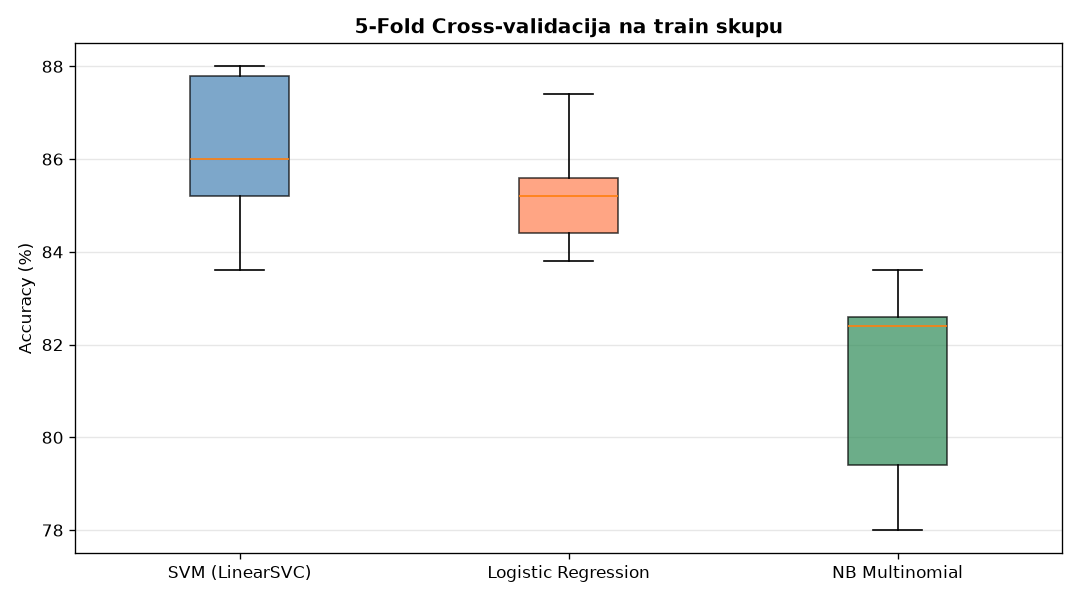
\includegraphics[width=0.75\textwidth]{18_cross_validation.png}
    \caption{5-Fold Cross-validacija na train skupu (top 3 modela)}
    \label{fig:crossval}
\end{figure}

\begin{table}[H]
\centering
\caption{Rezultati 5-Fold Cross-validacije na train skupu}
\begin{tabular}{lcc}
\toprule
\textbf{Model} & \textbf{CV Accuracy} & \textbf{Std. devijacija} \\
\midrule
SVM (LinearSVC)     & 86.12\% & $\pm$ 1.65\% \\
Logistic Regression & 85.28\% & $\pm$ 1.23\% \\
NB Multinomial      & 81.20\% & $\pm$ 2.13\% \\
\bottomrule
\end{tabular}
\end{table}

Cross-validacija na train skupu daje znatno više rezultate ($\sim$86\%) nego evaluacija
na test skupu ($\sim$72\%). Razlika od $\approx$14 pp ukazuje na određeni stepen
overfittinga — modeli se bolje snalaze unutar train distribucije. Mala standardna
devijacija (1.2–2.1\%) znači da su modeli stabilni. NB ima najveću varijabilnost
($\pm$2.13\%), dok je LR najstabilniji ($\pm$1.23\%).

\subsection{Najvažnije reči po autoru (SVM koeficijenti)}

\begin{figure}[H]
    \centering
    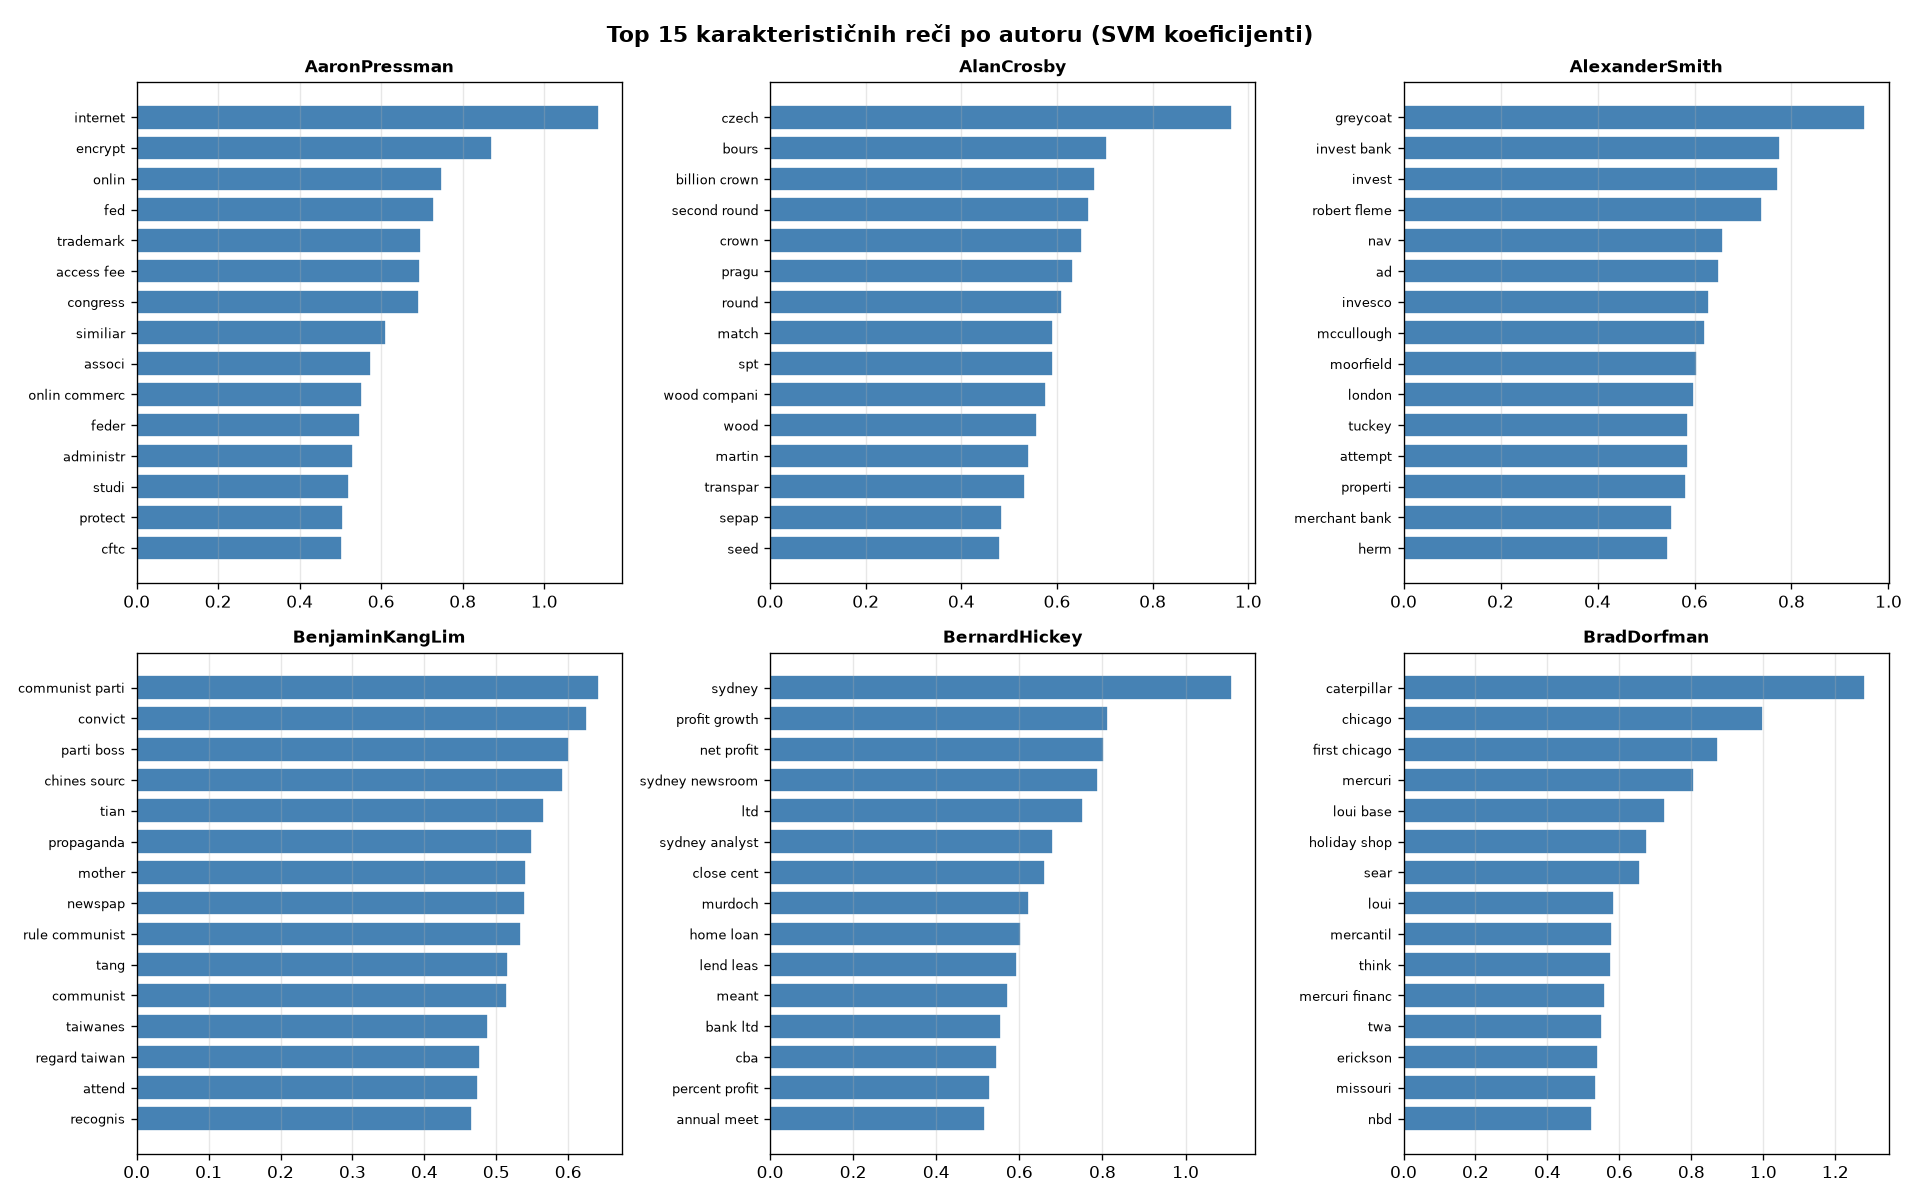
\includegraphics[width=\textwidth]{19_top_reci_svm.png}
    \caption{Top 15 karakterističnih reči za 6 autora — SVM koeficijenti}
    \label{fig:top_reci}
\end{figure}

SVM koeficijenti otkrivaju koje reči model smatra najkarakterističnijim za svakog autora.
Autori sa jedinstvenim temama (KarlPenhaul — ratni izveštač, FumikoFujisaki — Japan)
imaju visoko specifične top reči koje se ne pojavljuju kod drugih autora, što direktno
korelira sa njihovim visokim F1 skorovima. Autori koji pišu o azijskim tržištima
dele sličan vokabular (china, hong, kong, beijing), što ih čini međusobno nerazlučivima.

\subsection{Finalno poređenje modela}

\begin{figure}[H]
    \centering
    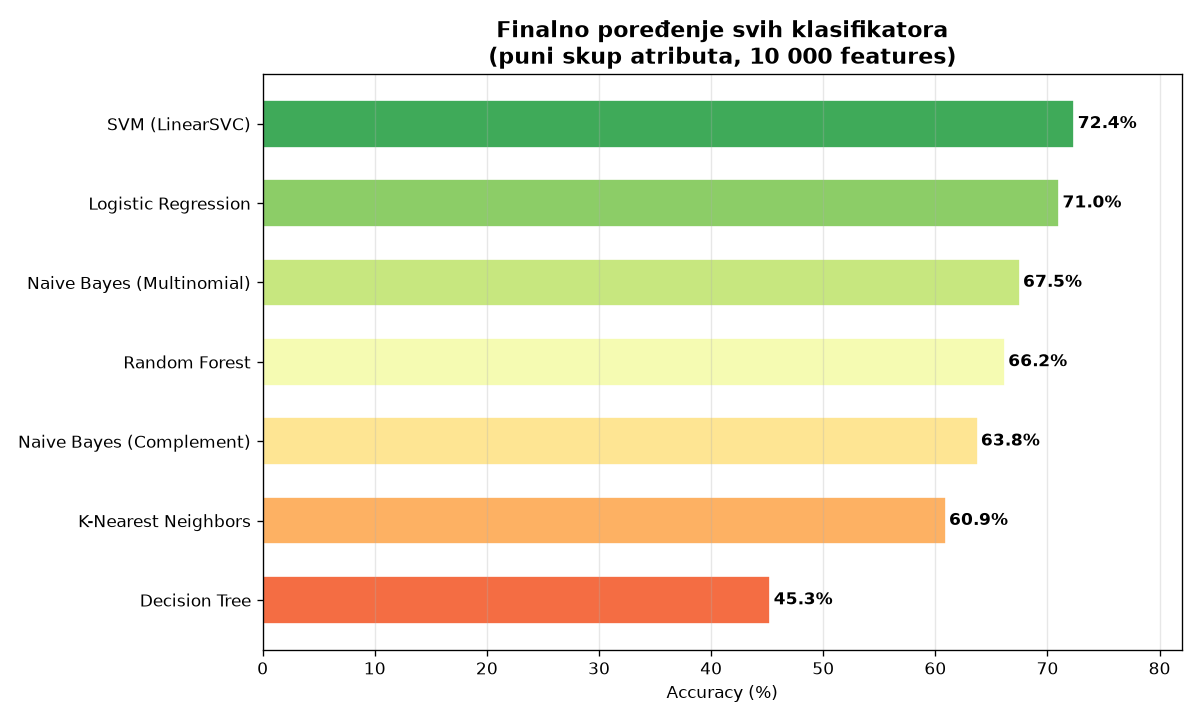
\includegraphics[width=0.85\textwidth]{20_finalno_poredenje.png}
    \caption{Finalno poređenje svih klasifikatora na punom skupu atributa}
    \label{fig:finalno}
\end{figure}

% ============================================================
%  8. ZAKLJUČAK
% ============================================================
\section{Zaključak}

U ovom radu primenjeno je istraživanje podataka na Reuters C50 dataset koji
sadrži 5000 novinskih članaka od 50 autora Reuters agencije. Problem klasifikacije
autora teksta je rešen primenom 7 algoritama na 3 skupa TF-IDF atributa (ukupno 21 model).

\textbf{Ključni nalazi:}

\begin{enumerate}
    \item \textbf{Najbolji model} je \textbf{SVM (LinearSVC)} sa \textbf{72.4\%}
    tačnosti na punom skupu od 10 000 TF-IDF atributa (unigrami + bigrami).
    Logistička regresija je blizu sa 71.0\%.

    \item \textbf{Linearni modeli dominiraju} — SVM i LR su superiorniji od
    ansambla (Random Forest), stabla odluke i KNN-a. Ovo je tipično za
    TF-IDF reprezentacije gde je prostor visokih dimenzija linearno separabilan.

    \item \textbf{Povećanje broja atributa dosledno poboljšava sve modele},
    ali sa smanjenjem prirasta. Dobitak od 500 na 2000 atributa je veći
    nego od 2000 na 10 000, što sugeriše zasićivanje.

    \item \textbf{Postoje značajne razlike između autora}: FumikoFujisaki
    i KarlPenhaul se klasifikuju gotovo savršeno (F1 $>$ 0.97), dok ScottHillis
    i JaneMacartney imaju F1 $<$ 0.30. Teški autori su uglavnom dopisnici
    koji pokrivaju iste teme (azijska tržišta) i dele sličan vokabular.

    \item \textbf{Cross-validacija} pokazuje stabilnost modela ($\pm$1–2\%)
    uz razliku od $\sim$14 pp između train CV ($\sim$86\%) i test tačnosti ($\sim$72\%),
    što ukazuje na određeni nivo overfittinga.

    \item \textbf{Preprocesiranje} je smanjilo broj reči za 45.5\%, uklanjajući
    šum i zadržavajući semantički bitne termine. Ovo je ključan korak koji
    direktno utiče na kvalitet klasifikacije.
\end{enumerate}

\textbf{Moguća poboljšanja:}
\begin{itemize}
    \item Primena neuronskih mreža (BERT, DistilBERT) za dublje semantičke reprezentacije
    \item Hiperparametarska optimizacija (Grid Search / Bayesian Optimization)
    \item Proširenje skupa atributa stilometrijskim karakteristikama
    (prosečna dužina rečenice, raznovrsnost vokabulara, upotreba interpunkcije)
    \item Primena ansambla top modela (SVM + LR + NB Voting Classifier)
\end{itemize}

% ============================================================
%  LITERATURA
% ============================================================
\newpage
\section*{Literatura}
\addcontentsline{toc}{section}{Literatura}

\begin{enumerate}
    \item Lichman, M. (2013). \textit{UCI Machine Learning Repository}.
    University of California, Irvine.
    \url{https://archive.ics.uci.edu/dataset/217/reuter+50+50}

    \item Pedregosa, F. et al. (2011). \textit{Scikit-learn: Machine Learning in Python}.
    Journal of Machine Learning Research, 12, 2825–2830.

    \item Bird, S., Loper, E., \& Klein, E. (2009).
    \textit{Natural Language Processing with Python}.
    O'Reilly Media.

    \item Manning, C. D., Raghavan, P., \& Schütze, H. (2008).
    \textit{Introduction to Information Retrieval}.
    Cambridge University Press.

    \item Porter, M. F. (1980). \textit{An algorithm for suffix stripping}.
    Program, 14(3), 130–137.

    \item Van der Maaten, L., \& Hinton, G. (2008).
    \textit{Visualizing Data using t-SNE}.
    Journal of Machine Learning Research, 9, 2579–2605.
\end{enumerate}

\end{document}
